\documentclass [11pt, a4paper]{report}

\usepackage[english]{babel}
\usepackage[utf8]{inputenc}

%\usepackage[lofdepth,lotdepth]{subfig}
\usepackage{graphicx}
\graphicspath{{images/}}

\usepackage{float}
\usepackage{subfig}

\usepackage{url}
\usepackage{xspace}

\usepackage{listings}
\usepackage{multirow}

%************************************************************
% Algotithms settings
%************************************************************
\usepackage[ruled,vlined]{algorithm2e}
\SetKwFor{On}{on}{}{}
\SetKwFor{Thread}{thread}{}{}
\SetKwFor{DoWithProbability}{with probability}{do}{}
\SetArgSty{textrm}

\SetKw{NONE}{none}
\SetKw{AND}{and}
\SetKw{OR}{or}
\SetKw{NOT}{not}
\SetKw{TO}{to}
\SetKw{FROM}{from}
\SetKw{Init}{init}
\SetKw{Wait}{wait}
\SetKw{Send}{send}
\SetKw{Receive}{receive}

\SetKwComment{Comment}{\%~~}{}
\SetCommentSty{textit}


\begin{document}

\newcommand{\cloudcast}{\emph{CLOUDCAST}}
\newcommand{\cyclon}{\emph{CYCLON}}
\newcommand{\cloud}{\emph{cloud}}
\newcommand{\amazonsss}{\emph{Amazon S3}}
\newcommand{\ptop}{\emph{peer-to-peer}}
\newcommand{\gossip}{\emph{gossip}}
\newcommand{\epidemic}{\emph{epidemic}}
\newcommand{\peersampling}{\emph{peer sampling}}
\newcommand{\rumormongering}{\emph{rumor mongering}}
\newcommand{\antientropy}{\emph{anti entropy}}
\newcommand{\descriptors}{\emph{descriptors}}
\newcommand{\descriptor}{\emph{descriptor}}

%%************************************************************
%% Commands used in algorithms
%%************************************************************
\newcommand{\deltacyclon}{$\delta cyclon$}
\newcommand{\deltaAntiEntropy}{$\delta antientropy$}
\newcommand{\deltaRumorMongering}{$\delta rumormongering$}
\newcommand{\view}{\emph{view}}
\newcommand{\views}{\emph{views}}
\newcommand{\request}{\emph{request}}
\newcommand{\reply}{\emph{reply}}
\newcommand{\msize}{size}
\newcommand{\mget}{get}
\newcommand{\mput}{put}
\newcommand{\mclear}{clear}
\newcommand{\mremove}{remove}

\newcommand{\GET}{\emph{GET}}
\newcommand{\GETALL}{\emph{GETALL}}
\newcommand{\PUT}{\emph{PUT}}
\newcommand{\PUTALL}{\emph{PUTALL}}
\newcommand{\REQUEST}{\emph{REQ}}
\newcommand{\REPLY}{\emph{RSP}}
\newcommand{\VIEW}{\emph{VIEW}}
\newcommand{\PUSH}{\emph{PUSH}}
\newcommand{\PULL}{\emph{PULL}}
\newcommand{\PUSHPULL}{\emph{PUSH-PULL}}


%************************************************************
%  Inizio Prima Pagina
%************************************************************
\begin{titlepage}
\begin{center}
\LARGE
UNIVERSIT\`A DEGLI STUDI DI TRENTO\\
\large
Facolt\`a di Scienze Matematiche, Fisiche e Naturali\\
\begin{figure}[htbp]
\centering

\includegraphics[width=80pt,height=80pt]{unitn_logo.png}
\end{figure}
% \thispagestyle{empty}
\large
Corso di Laurea Magistrale in Informatica\\
\rule{\linewidth}{0.5mm}
\ \\ \ \\
Tesi\\
\ \\ \ \\ \ \\ \ \\
\Large
CloudyPeer: a Framework for Developing Cloud-Aware, Peer-to-Peer
Applications
\end{center}

\ \\ \ \\ \ \\ \ \\ \ \\ \ \\ \ \\ \ \\ \ \\ \ \\ \ \\
\large
\flushleft \large Relatore: \hspace{\stretch{2}} \large Laureando:\\
\large prof. Alberto Montresor   \hspace{\stretch{1}} \large Andrea Zito\\
\flushleft \large Correlatore:\\
\large prof. Luca Abeni
\normalsize
\ \\ \ \\ \ \\
\begin{center}
 Anno Accademico 2010-2011
\end{center}
\end{titlepage}
%************************************************************
%  Fine Prima Pagina
%************************************************************

{
  \baselineskip=13pt
  \tableofcontents
}

\chapter{Introduction}
\textit{Cloud computing} represents an important tecnology in the
modern Internet era. The promises of virtually infinite storage
capacity and computation resources, in conjunction with the fact that
costs are computed with a \textit{pay-per-use} model, make it very
appealing to small companies. Recent years have seen the rise of Internet based
\textit{start-up}, which, by exploiting the \cloud, have the opportunity
to compete on equal terms with software giants like Microsoft
and Google. A representative example is Dropbox which, relaying on
\amazonsss service, has become, in a very short time, a dominant player
in the sector of file storage.

The increasing interest in \cloud computing has resulted in the
reduction of the appeal of another trend of the last decade: the \ptop
paradigm. This model displays similar characteristics with respect to
the \cloud, but, at the same time, it does presents substantial
differences. The
cost of operating a \ptop architecture is virtually non-existent,
making it extremely desirable from an economic point of view. At the
same time, however, the \cloud offers a much higher availability,
making it a more appropriate solution for those businesses which are not
well suited to the \textit{best effort} philosophy of \ptop.

Both the academic community and the commercial world have tried to mix
the two approaches with the intent of achieving the above mentioned
properties at the same time. The two main strategies which have
emerged see the
addition of peers to a centralized solution on one side and the
extension of existing \ptop systems with elastic computing nodes on
the other.
For example, the first tactic has been exploited in
video-on-demand~\cite{PeerAssistedVoD} and file
distribution~\cite{BitTorrentRobustness}~\cite{AmazingStore}
applications where storage
and bandwidth costs are reduced, when availability
constraints allow it, by off-loading to clients the burden of
providing the service. The second strategy, instead, has been applied
to bulk-synchronous content distribution~\cite{AngelsInCloud}
and online backup~\cite{PeerAssistedOnlineDataBackup} scenarios to
satisfy requirements beyond the reach of a \ptop system.

A novel approach to the problem, which greatly differentiates itself
from the previous examples, has been recently proposed. The
illustrated architecture, called \cloudcast~\cite{Cloudcast}, sees an
integration of the \cloud in all the level of the \ptop system, making
the two of them a coherent entity. To achieve this task, \cloudcast
exploits a number of standard \ptop protocols, some of which have been
modified to take into account the new requirements. The number of
entities involved in the architecture make developing applications
based on it a quite long and error-prone task. Other than focusing on
the target domain, a lot of work must go into designing and implementing
the base infrastructure.

This kind of problem is indeed true for many \ptop oriented solutions
and has been partially solved via the creation of multiple frameworks
by the academia~\cite{AntHill}~\cite{P2PFramework},
enterprise bodies~\cite{JXTA}~\cite{dotNETp2p} and open-source
projects~\cite{GNUnet}. The general idea is to simplify the burden
imposed on the developer, either by providing domain specific solutions
or by offering the building blocks needed to design a complex system.

\paragraph{Contributions} In this thesis we present the efforts that
have been made to develop a working implementation of the \cloudcast
infrastructure. Furthermore we describe and evaluate the improvements
that have been produced while performing the task. The second half of
the work deals with the analysis and the implementation of
\cloudypeer, a general \textit{Java} framework which, exploiting \cloudcast,
provides the means to easily build applications focused on the content
diffusion scenario. In conclusion, a practical example is presented in
the form of a \textit{RSS} delivery software, called \cloudyrss, which
has been developed to prove the viability of the proposed approach and
will be used, in future works, to evaluate it in a real context.

\chapter{\cloudcast}

As has been illustrated in the introduction, many strategies aimed at
augmenting \ptop systems with \cloud entities, have been
proposed. Even though they embrace profoundly different philosophies,
a distinctive element common to all of the surveyed methods
is that the \cloud lives on a different conceptual level with respect
to the \ptop system: the two components work together to achieve the
final goal, but they are not integrated in an unified architecture.

In this respect \cloudcast \cite{Cloudcast} represents a novel approach
of \emph{peer-assisted} distributed computing, tailored for content
distribution scenarios. Indeed all the functionality of the system are
tightly bound to the \cloud: not only the actual information
dissemination, but also the entire management of the \ptop network
(including node bootstrap, membership and topology management). There is
no need for \emph{active} elastic computing instances, as the
whole design is conceived to be supported by a \emph{passive} storage
service such as \amazonsss.

Thanks to this central role of the \cloud and the way the topology is
maintained, \cloudcast is able to approximate a constant number of accesses
to the storage service independently of the network size, while
being able to scale in both directions. A small system characterized by
few users will mostly exploit the \cloud to deliver informations. As
more users join, the load will be spread on the
\ptop network. In all cases the amortized cost of the storage service
will remain under control: even better, the cost per user will
decrease as the user base increases.

\section{Architecture}
From an architectural viewpoint, \cloudcast is composed by two
well known \gossip protocols:
\peersampling \cite{GossipPeerSampling}
and \epidemic broadcast \cite{EpidemicAlgorithms}.
The former is responsible of bootstrapping and maintaining the topology,
whilst adjusting the \cloud contact rate as a function of the number
of nodes. The latter takes care of the actual information
dissemination, using the first as a source of peers, and it is in turn
divided into two instances: \antientropy and \rumormongering.

An overview of \cloudcast's architecture is shown in
Figure~\ref{fig:cloudcast-architecture}. The labeled arrows highlight the
interactions between the various components from the point of view of a
single peer.

\begin{figure}
  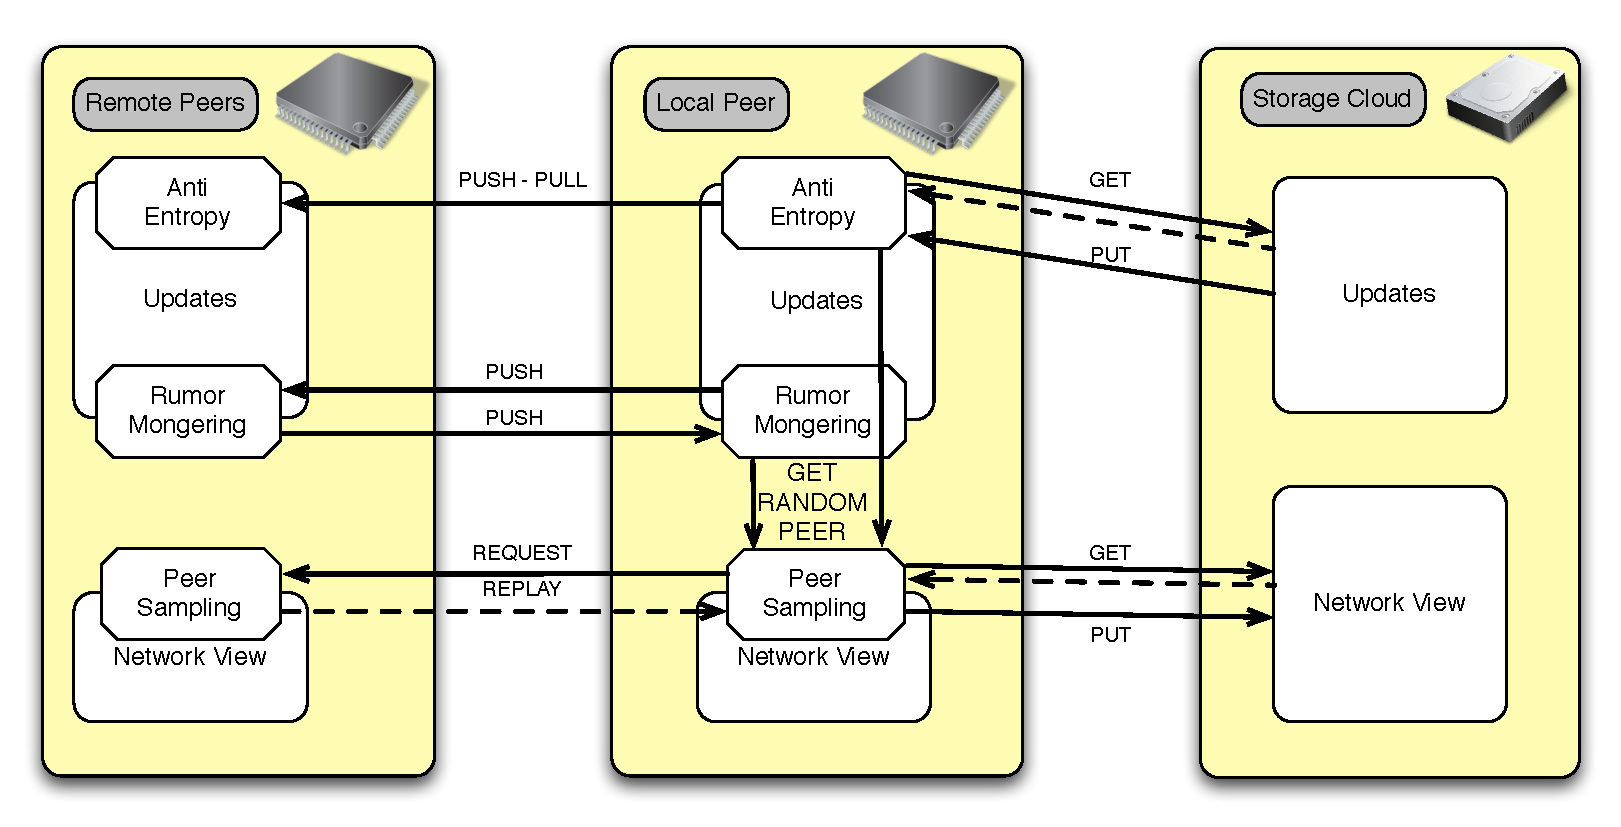
\includegraphics[width=\textwidth]{cloudcast-architecture.pdf}
  \caption{\cloudcast architecture summary highlighting component
    interactions from the point of view of a single peer}
  \label{fig:cloudcast-architecture}
\end{figure}

As can be seen, both the peers and the \cloud maintain the same set of
information (updates on information to be diffused and partial view of
the system membership): the only difference lays in the fact that the latter
lacks any active involvement.
\ \\
In the following sections we analyze in detail the protocols
forming the \cloudcast architecture with a particular focus on the
\cloud interactions.

\section{Peer Sampling}
The \peersampling protocol at the heart of \cloudcast is built upon
\cyclon \cite{CYCLON}, a well known \peersampling \gossip protocol
which has proven to provide good randomization and churn resistance,
while at the same time approximating a constant node in-degree.

In \cloudcast each node maintains a partial \view\ of the entire system
in the form of node \descriptors. Periodically each node selects
a partner to execute an information exchange, during which old
\descriptors are potentially removed (to take care of failed or
otherwise unresponsive nodes), new ones are created (to notify that the
peers involved in the exchange are still active) while existing
entries are shuffled (to satisfy the randomization property which
guarantees the network graph connectivity).

The protocol relays on a set of parameters which directly influence its
performances. Firstly the ones inherited by \cyclon: the period of
the information exchange (\deltacyclon), the size of the partial
\view\ of the network known by each peer ($c$) and the length
of the message exchanged in each cycle ($g$). Furthermore
\cloudcast introduces the variable $k$ which is used to tune the
\cloud contact frequency.

Algorithm \ref{algo:cloudcast_original_active} shows the operations
performed by the active thread of the protocol, while algorithms
\ref{algo:cloudcast_original_passive_peers} and
\ref{algo:cloudcast_original_passive_cloud} illustrate the actions
executed in response to events by the passive thread (for a clearer
explanation of the changes introduced, with respect to the original
\cyclon protocol, refer to \cite{Cloudcast}).

% Insert original cloudcast's protocol algorithms
\input algorithms/cloudcast_peersampling_algo

Every \deltacyclon\ each node fills its local \view\ by reinserting
entries sent in the previous cycle (block 1), thus
maximizing the out-degree and at the same time preventing loosing
entries (the rationale behind this statement will be evident later).
In code block 2 all the \descriptors in the \view\ are aged
by 1. Next, in block 3, the oldest \descriptor (the one with
the maximum timestamp) is selected and removed from the \view: this
has the effect of clearing the overlay from old entries associated to
failed nodes.

At this point the behavior of the protocol differs in function of the kind
of peer selected in the previous step. In case of a \cloud entry, a
request is sent to the storage service for the key ``view''
(block 4). If instead the selected partner is a normal peer,
a \request\ object containing up to $g$ \descriptors (removed from the
local \view) is created and consecutively sent to the counterpart
(block 5-6). The number of entries contained in
the \request\ is stored in the variable $res$ and has the purpose of
specifying an upper bound on the number of \descriptors expected as a
response by the remote peer.

Algorithm~\ref{algo:cloudcast_original_passive_peers} shows the actions
performed in response to peers related
events. Blocks 7-9 handle requests generated by
the active thread. Peers shuffle the local \view\ by randomly exchanging
\descriptors with the ones present in the \request\ object
and at the same time generating a \reply\ containing the removed local
entries. The $res$ variable plays an important role here: if the peer
was in the middle of an active cycle, the constraint of filling the
local \view\ for as much as $c - res$ elements would guarantee that, when
the counterpart's \reply\ will be received, there will be enough free
space to hold its content.

In block 10 it can be seen the procedure which terminates an
active cycle: peers just absorb the \reply's entries and clear the
space reservation by assigning 0 to $res$.

Up until here, apart from the minor divergence in the active
thread, the protocol closely follows \cyclon. The novelty of the
approach can be appreciated in
algorithm~\ref{algo:cloudcast_original_passive_cloud}.
Here peers simulate an entire dialogue with the \cloud (which being
a passive entity cannot take part in the protocol
itself). Block 11 and 12 emulate respectively
the construction of a local \request\ and a remote \reply. Whereas
the former is built accordingly to the previously described procedure,
the formation rules of the latter are more complex. Indeed
block 12 is the responsible for the maintenance of the
expected number of \cloud \descriptors. The \reply\ is populated with
a variable number of \cloud entries in the interval [0,2] in function
of the current contact frequency of the storage service.

To perform this adaptive scheme, \cloudcast exploits the modification
timestamp (represented by $t$ in the algorithm) associated to each
object by the storage service. If it indicates that the \cloud is not
being contacted too frequently (i.e. $now() - t >$ \deltacyclon $* k$)
then a first entry is added. Furthermore if it shows that the contact
rate is too sporadic (i.e. $now() - t >$ \deltacyclon $/ k$) then a
second entry is included.
The aforementioned parameter $k$ is adopted here to tune the time
window defining the target contact frequency: values tending towards 1
will result in an always more narrower window peaked on \deltacyclon\
(i.e. only one contact per each \cyclon cycle is acceptable) while
higher values allow more relaxed constraints.

Once the \request\ and \reply\ are completely formed they are merged
respectively with the \cloud and the local \view. This is carried out by
blocks 14 and 15. At this point the
simulated cycle is almost completed: both the \views are shuffled and new
\descriptors are added. The only remaining action to be performed by
the peer is to write the modified \view\ to the storage cloud
(block 15).

\section{Epidemic Broadcast}
\label{sec:epidemicbroadcast}
As previously mentioned, the actual information dissemination is
carried out by two \epidemic broadcast protocols. The
\antientropy instance is run periodically (every \deltaAntiEntropy)
and is responsible to
reduce differences between peers: asymptotically this guarantees that
all node receive all the updates. To fulfill this promise the
protocol have to be fairly expensive in terms of bandwidth, as it
requires the full set of data to be exchanged by involved
peers. Having to take into account the \cloud alongside standard peers,
the original algorithm by Demers~\cite{EpidemicAlgorithms} must be
adapted to the current scenario:
algorithm~\ref{algo:cloudcast_antietropy} shows the modified pseudo
code.
In block (ae1) the \cloudcast \peersampling protocol is queried
for a random peer currently in the \view. Blocks (ae3) and (ae4)
implement the original difference resolution between peers, while
block (ae2) adds the interaction with the \cloud.
All the strategies discussed in the paper are supported by
\cloudcast and are reflected in the code by the parameter
\emph{strategy}.

% Insert anti entropy protocol
\input algorithms/cloudcast_antientropy_algo.tex

Having solved the problem of comprehensively diffuse updates, the last
protocol in the architecture deals with the complementary task of
quickly and efficiently distribute updates in a \emph{reactive} fashion. This is the
role played by the \rumormongering \epidemic broadcast.
In \rumormongering, peers are initially \emph{ignorant}. Whenever they
receive an update this becomes an \emph{hot-rumor}. Peers holding an
\emph{hot-rumor}
select, every \deltaRumorMongering time units, a random peer in the current
topology and send (\emph{push}) the update to it. The rumor ceases to
be hot according to different strategies~\cite{EpidemicAlgorithms},
 all of which are applicable with \cloudcast.
As can be seen in figure~\ref{fig:cloudcast-architecture}, \rumormongering\
does not interact directly with the \cloud, but involves only normal
peers.

The rationale behind this choice is that, by its very nature, the
protocol is \emph{reactive} and hence not applicable to a
\emph{passive} entity. Furthermore \cloud \descriptors are
excluded from the random selection of peers to avoid that the
introduction of an update results in an \emph{explosion} of contacts
to the storage service. This does not affect the quality of the
information dissemination, as the \cloud will in any case receive the
news thanks to the \antientropy instance.

The algorithm for this protocol is omitted, as it does not need any
modification to be adopted in \cloudcast; for more information on the
implementation refer to the original paper\cite{EpidemicAlgorithms}.

\section{Simulation results}
\cloudcast has been subjected to many simulations performed with the event
driven version of the \textit{PeerSim P2P Simulator}\cite{Peersim}.
In this section
are proposed some of the obtained results with the purpose of defining
a comparison framework against which evaluate the performance of the real
implementation. The paper~\cite{Cloudcast} from which these plots are
taken offers an in-depth analysis of the performances of the system
which is not covered here, as it is not the focus of this work.

Table~\ref{tbl:cloudcast-sim-parameters} provides an overview of the
parameters used to perform the simulations.

\begin{table}[H]
  \centering
  \begin{tabular}{|l|l|l|}
  \hline
  Parameter & Value & Meaning \\
  \hline
  \hline
  $n$ & $2^6$--$2^{16}$ & Total number of peers \\
  \deltacyclon & 10s & Cycle length of \cyclon \\
  \deltaRumorMongering & 1s & Cycle length of \rumormongering\\
  \deltaAntiEntropy & 10s & Cycle length of \antientropy\\
  $c$ & 20 & View size \\
  $g$ & 5 & \cyclon message size \\
  $strategy_{ae}$ & \PUSHPULL & Strategy adopted by \antientropy\\
  $strategy_{rm}$ & \emph{Blind/Coin} & Strategy adopted by \antientropy\\
  $p_{\emph{rumor}}$ & 0.2 & Probability of rumor ceasing being hot \\
  $k$ & 4 & \cloudcast threshold parameter \\
  \hline
  \end{tabular}
  \caption{Parameters used in the simulations.}
  \label{tbl:cloudcast-sim-parameters}
\end{table}


\subsection{Peer Sampling}
Considering the importance of the role covered by the
\peersampling protocol in the \cloudcast architecture, it is appropriate
for it to represent the first evaluation candidate.

Figure\ref{fig:cloudcast-sim-oscillating-indegree} shows the
\cloud in-degree as it changes during the course of $4$ simulated
days. Each day starts with $0$ peers in the network and sees them grow
until the peak of $500$ is reached at noon. At this point the network size starts
the descending phase, which culminates at midnight with the complete removal of all
peers. As can be seen in the zoomed-in view shown in
figure~\ref{fig:cloudcast-sim-oscillating-indegree-detail}, the
in-degree of the cloud oscillates around the target value $c$ and it is
constantly adjusted to reflect the variations of the network size.

\begin{figure}[H]
  \centering
  \subfloat[][Global view]{
    \hspace{-70pt}
    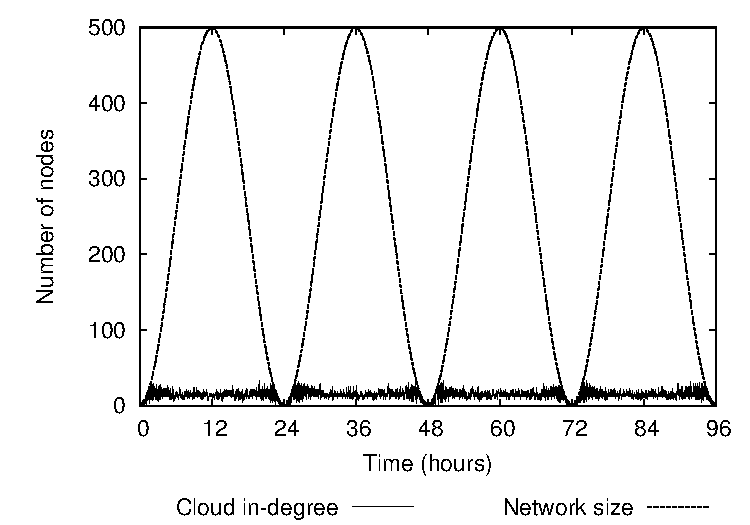
\includegraphics[width=240pt]{cloudcast-sim-oscillating-indegree.pdf}
    \label{fig:cloudcast-sim-oscillating-indegree}
  }
  \subfloat[][Detail of a simulated day]{
    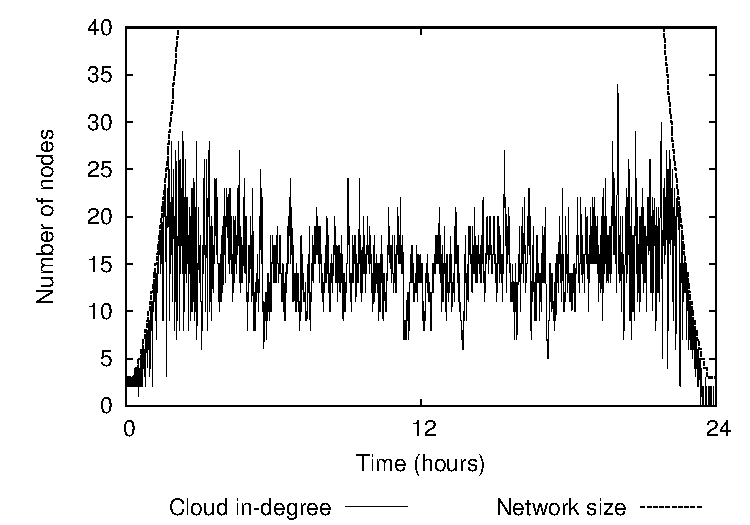
\includegraphics[width=240pt]{cloudcast-sim-oscillating-indegree-detail.pdf}
    \label{fig:cloudcast-sim-oscillating-indegree-detail}
  }
  \caption{\emph{Cloud} in-degree for a network oscillating daily
    between $0$ and $500$ nodes.}
  \label{fig:cloudcast-sim-oscillating-indegree-global}
\end{figure}

Moving our attention to the impact of the \peersampling protocol on
the \cloud, figure~\ref{fig:cloudcast-sim-loads} verifies the assertion
that the system scales well with the growing of the network size. The
plot relates the aggregated number of \cloud contacts, over the course
of the day, with different network sizes. As can be seen, small topologies
tend to relay for the most part on the \cloud, while the loads
decrease and stabilize for larger ones.

\begin{figure}[H]
  \centering
  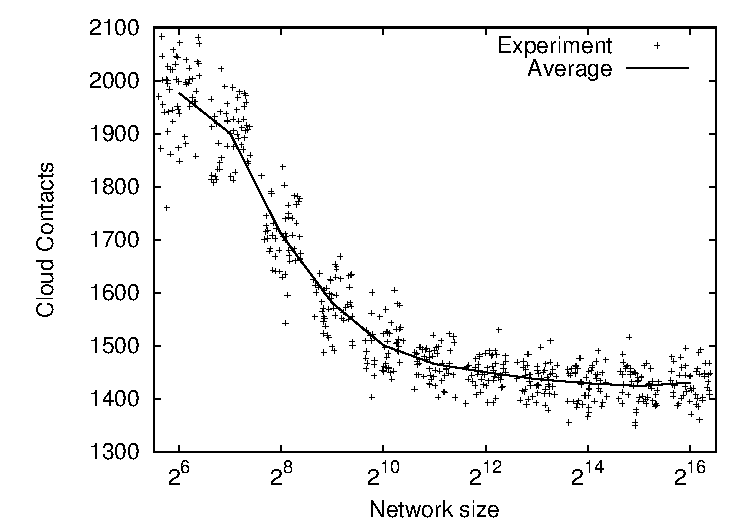
\includegraphics[width=.7\textwidth]{cloudcast-sim-loads.pdf}
  \caption{Storage \cloud load for different network sizes.}
  \label{fig:cloudcast-sim-loads}
\end{figure}

\subsection{Epidemic Broadcast}
For what concerns the \epidemic broadcast components of
\cloudcast, an interesting measurement is the delay with which peers
receive updates. This data is proposed in
figure~\ref{fig:cloudcast-sim-delays} for different network sizes.
Figure~\ref{fig:cloudcast-sim-oscillating-delays} instead keeps track
of the delays in a dynamic scenario of an oscillating network of
$500$ nodes. The dashed lines represent the average delay for each
update computed by the following rule: delta between the receiving
time of update $m$ by peer $i$ and the issuing time of update $m$, if
peer $i$ was active when update $m$ was issued; delta between the
receiving time of update $m$ by peer $i$ and the joining time of peer
$i$ otherwise.

\begin{figure}[H]
  \centering
  \subfloat[][Delays for different network sizes]{
    \hspace{-70pt}
    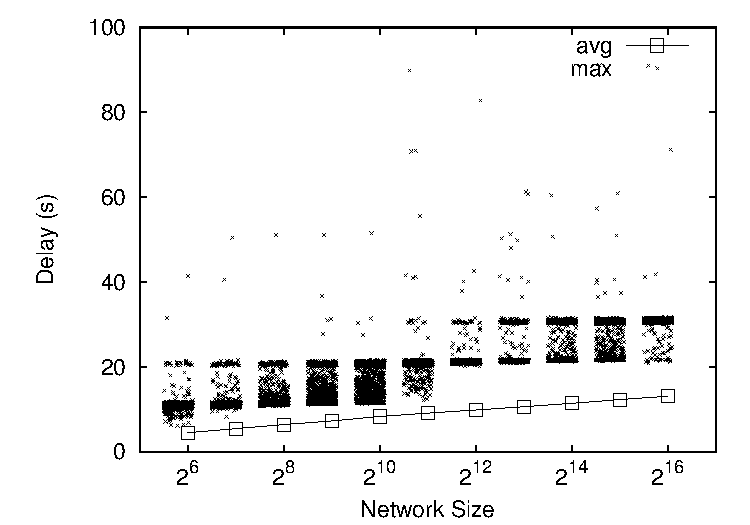
\includegraphics[width=240pt]{cloudcast-sim-delays.pdf}
    \label{fig:cloudcast-sim-delays}
  }
  \subfloat[][Progressive delays in a dynamic scenario]{
    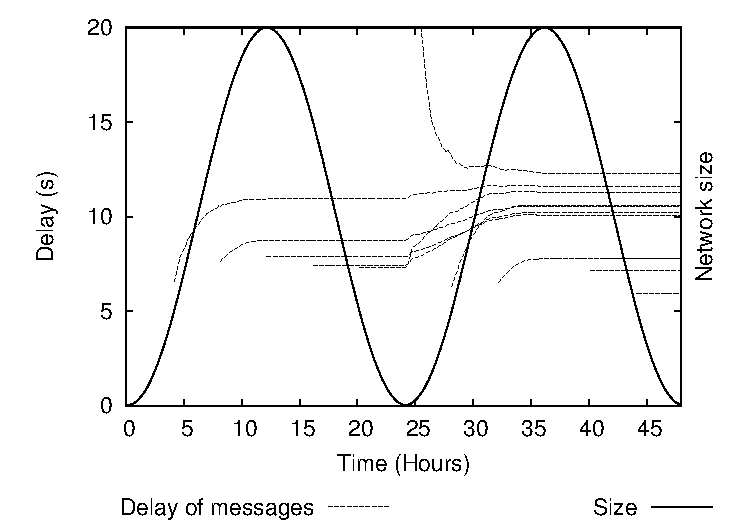
\includegraphics[width=240pt]{cloudcast-sim-oscillating-delays.pdf}
    \label{fig:cloudcast-sim-oscillating-delays}
  }
  \caption{Delays in messages diffusion for fixed and oscillating networks}
  \label{fig:cloudcast-sim-globa-delay}
\end{figure}

\section{Additions to the Peer Sampling protocol}
\label{sec:cloudcast-additions}
The results presented in the previous section prove that
\cloudcast is a stable protocol capable of forming and maintaining a
connected topology satisfying the constraints on the \cloud contact
rate. However,
the tricks that has been used by the simulation to emulate the interaction
with the storage service, hide some of the problem that real
implementations must face. For instance, in the real world, the
\cloud storage could be unreachable due to overload of the provider
or more realistically due to failure on the peer's end. Remembering
that peers selected as target in the active cycle are removed from the
local \view, this means that a temporary error contacting the
storage service could result in the loosing of all the
\cloud \descriptors in the network.

Even without considering this scenario, a recovery mechanism able to
re-establish the correct behavior is needed to guarantee the stability
of the protocol under any circumstance (e.g. abruptly removal of large
part of the topology).

To resolve this issue, during the course of this work, the
\peersampling protocol has been expanded with some minor additions.

% Insert additions cloudcast's protocol algorithms
\input algorithms/cloudcast_peersampling_algo_additions

Algorithm~\ref{algo:cloudcast_addition_active} shows the
supplementary actions performed by the modified \cyclon active thread,
while algorithm~\ref{algo:cloudcast_addition_passive} reports
the extra operations carried out by the passive routines.

Two variables have been added to reflect the new states of the protocol:
$bakC$, used to store a back-up copy of the \cloud \descriptor selected
as target, and $T$, which keeps track of the last time any peer
contacted the \cloud.

Blocks a1, a4 and a8 implement the safeguard on
\cloud entries. Whenever an active cycle involving the storage
service starts, the corresponding \cloud \descriptor is saved in the
variable $bakC$ (block a4). When the remote \view\ is received,
triggering the procedure responsible for the tuning of the
\cloud contact rate, the saved entry can be cleared, as the risk of
losing it is ceased (block a8). If, instead, the reply from the storage
service is not received in time for the next cycle, the saved entry is
reinstated (block a1). Since this check is done after the selection and
consequential removal of the target peer, it is guaranteed that the local
\view\ has a free spot for the backed-up \cloud \descriptor.

The next addition with respect to the original protocol regards the
recovery mechanism. In block a3 the variable $T$, containing the
timestamp of the last storage service contact, is tested against the
threshold parameter \maxsilence: in case of failure a new
\cloud entry is added to the local \view\ with probability
\spawnprob. The variable $T$ is updated every time the
\cloud is selected as target for the active cycle (block a4) and is
piggybacked on all the peers messages (blocks a5 and a6). When any
such message is received, the variable $T$ is confronted with the
remote counterpart and, if appropriate, updated (blocks a6 and a7).

Thanks to this strategy, if all the \cloud \descriptors are removed
from the topology, the ``black-out'' lasts for as much as
\maxsilence. The probabilistic insertion avoids a sudden explosion of
\cloud entries, while the usual tuning mechanism takes care of
restoring the optimal in-degree.

Block a2 concludes the analysis of the protocol's modifications. This
portion of pseudo code implements a simple check that forces the
addition of a \cloud entry in case of an empty \view. This simple
check is enough to guarantee that peers which remain cut off from the
topology can automatically rejoin the network.

\chapter{\grapes}
\grapes (Generic Resource Aware P2P En- vironment for Streaming) is a
toolkit providing a set of \textit{generic} and \textit{reusable}
components for the development of \ptop application focused on
streaming scenarios. The fundamental philosophy behind its design is
to support as many different environment as possible while keeping at
a minimum the restrictions imposed on the applications employing it.
For these reasons it's implemented as a pure C library without any dependencies
on external libraries: as a result \grapes can be used on a variety
of systems, from high-power servers to embedded devices.

The functionality offered by the toolkit are divided into cleanly
separated modules:
\begin{itemize}
  \item \textit{Chunk Trading}, allowing to send/receive pieces of a
    media stream (called chunks);
  \item \textit{Chunk Buffer}, used to store the received chunks so
    that they can be forwarded to the other peers;
  \item \textit{Chunk ID Set} data type, that can be used to send
    signaling information about the received or needed chunks;
   \item \textit{Scheduling} functions, which can be used to decide
     which chunk to send/ask, to which peer;
   \item \textit{Network Helper}, used by the other modules and the
     applications to delegate network related tasks;
   \item \textit{Peer Set} data type, to store information about the
     nodes connected to a specific peer in the overlay (the so called
     neighbors);
   \item \textit{Peer Sampling} protocols, providing each peer with
     continuously up-to-date random samples of the entire population
     of peers.
\end{itemize}

The first four modules are not related to this work and thus will not
be covered here: for further information refer to the
\grapes paper~\cite{GRAPES}.

\ \\
The last three instead compose the fundamental blocks needed to build
the \cloudcast \peersampling protocol. The \textit{Peer Sampling} module
offers a simple implementation of \cyclon; the \textit{Peer Set}
features common set manipulation functions and support for
\textit{metadata}. In conclusion the \textit{Network Helper} greatly
simplifies the use of the network and promise the support for
\textit{NAT traversal} techniques.

In light of these facts, instead of re-implement all of the
infrastructure from scratch, it was chosen to use \grapes as a
starting point adding to it the missing components.
The rest of this chapter will cover in detail the work performed on
grapes during the course of this thesis.

\section{Groundwork}
The first issue which was identified during the initial analysis of
the toolkit was that some component (prominently the \textit{Peer
  Sampling}) were designed to support only one instance per
executable: global variables were used to maintain protocols states and
to act as buffers. Furthermore the \api did not exposed any mechanism
to select a specific instance to act on.

Such a design choice don't play well with the final aim of this work: it
would limit an application built upon it to take part in only a single
\peersampling instance. The problem was solved by \grapes authors by
having multi-process applications, where each single process is
responsible for a specific instance and communicates with other
via \emph{IPC} mechanism. Whereas this approach is both effective and
efficient when considering program written in a compiled language
such as C or C++, things rapidly changes when we shift attention to
languages requiring a \emph{virtual machine}: the aggregated memory
footprint of the application as a whole is dominated by the memory
required by the multiple \emph{VMs}. In these situations a better
approach is to keep all the application logic in a single executable
and possibly using \textit{threads} to ease the programming task.

Keeping this in mind, the first effort taken was to modify the
\emph{Peer Sampling} module to support concurrent instances. The
functions forming the high level \grapes's \api are explicitly written
to be re-entrant and should be consider thread safe, hence the only
real modification needed was the addition of execution contexts to
separate parallel instances. The task was accomplished in an
\emph{Object Oriented} inspired way: the state of each protocol was
collapsed in a C \emph{struct} which is passed as the first
argument of each \emph{Peer Sampling} \api's function thus identifying
the \emph{object} to act upon.

\ \\
Another side task which required a fairly large amount of time was the
debugging of the \emph{Peer Set}'s manipulation functions. The
first tests performed on a partial implementation of the modified
\cyclon shown odd result which greatly deviate from the simulated
behavior. After a thorough analysis a bug was found in the function
responsible for the insertion of node \descriptors in the \view.
Furthermore the \emph{Peer Set} \api was augmented with a number of
supplementary functions to manage the \textit{filling} and
\textit{sampling} of sets.

\section{Cloud Helper}
At this point the only feature \grapes missed in order to implement
\cloudcast \peersampling protocol was the support for the storage
service. A simple solution to the problem would have been to simply
relay on an external library and explicitly make use of it. Whereas
being quick and easy this strategy does not comply with the
portability requirement of the project and at the same time would have
limited the \cloud support to a single provider.

This is the rationale that lead to the introduction of the
\cloudhelper abstraction layer. This module, in line with the rest of
\grapes components, exports a simple \api (shown in
\ref{fig:grapes-cloudhelper}) which can be used by other
modules or by the final application.

\begin{figure}[H]
  \centering
  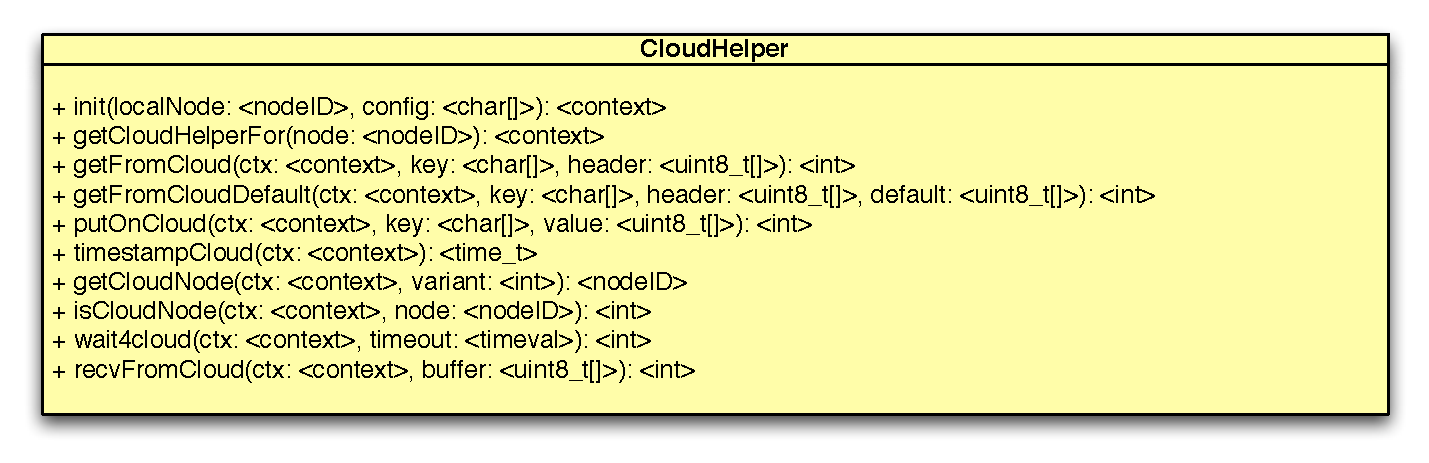
\includegraphics[width=\textwidth]{grapes-cloudhelper.pdf}
  \caption{Diagram of the \cloudhelper \api.}
  \label{fig:grapes-cloudhelper}
\end{figure}

As can be see the functionalities offered by the \api cover only the
basic \cloud operation and the support for metadata is limited to the
last modification time: indeed at the current state only those
functions needed for the \cloudcast implementation where
added.
Given that the purpose of the functions and their use is for the most
part self explanatory, in the following paragraphs it will be given
only a quick overview of them.
\emph{GetFomCloud} and \emph{getFromCloudDefault} are used to
query the \cloud for a specific \textit{key}. Both of them support the
addition of custom header to the reply to ease the processing
phase. In addition \emph{getFromCloudDefault} allows the caller to
set a default reply to be used in the event that the specified
\textit{key} is not present on the \cloud. Symmetrically
\emph{putOnCloud} takes care of updating the value of a specific
\textit{key}. These function all use plain bytes to represent
data (in the form of array of \textit{uint8\_t}) and their return
value indicates the state of the operation: $0$ is used to signal a
success while $1$ means that an error occurred while performing the
action. The \emph{timestampCloud} function is used to obtain the time
of the last modification associated to the most recent
\textit{completed} query. A query is considered \textit{completed}
when the associated response is read. This is done via the
\emph{recvFromCloud} function which stores the received data in the
specified buffer and return the number of bytes read. Application can
exploit the function \emph{wait4Cloud} to wait for the \cloud to
perform a query: a return value of $1$ indicates that the
operation was successful and the data can be read, $-1$ means that the
specified \textit{key} could not be retrieved (most likely because it's
unknown) and finally $0$ inform that some other error occurred.

The two functions \emph{getCloudNode} and \emph{isCloudNode} are used
to handle the interaction with the \textit{Peer Set} module: the
former creates new peer \descriptor using the \textit{variant}
parameter as the index of an imaginary \cloud \descriptor enumeration;
the latter instead is used to check if a specified \descriptor is
indeed referring the \cloud.

The remaining two functions are used to manage the \textit{execution
  context} of the \cloudhelper. \emph{GetCloudHelperFor} retrieve the
\textit{context} associated to a particular peer \descriptor: this
functionality is used by the \cloudcast \peersampling protocol to
fetch a configured \cloudhelper instance without requiring
modification to the current \grapes \textit{Peer Sampling} module
\api. \emph{CloudHelperInit} is the function responsible for the
creation and configuration of new \cloudhelper \textit{execution
  contexts}. Adhering to the convention in use by \grapes, this function
exploit an \textit{opaque} configuration string containing an
human readable representation of the parameters.

At the current stage the only parameter directly supported by the
\cloudhelper module is represented by the string ``\textit{provider}''
and it's used to select the actual implementation which will back the
newly created \textit{context}. Such implementation will be
responsible for parsing the remaining portion of the configuration
string.

During the course of this work two \cloudhelper implementation were
developed. The first is backed by \textit{Amazon Simple Storage
  Service} \cloud and it's based upon \textit{libS3}~\cite{LibS3}. The
second one uses a \textit{MySQL} database as storage and it
make use of \textit{MySQL Connector/C}~\cite{MySQLConnectorC}. Both
these libraries takes with them a number of dependencies and provide
synchronous operations (in contrast to the asynchronous paradigm used
by \grapes). Given the stringent restriction on dependencies and
\textit{threads} usage by the original project it was chosen not to
include the these \cloudhelper implementation directly in the code
base, instead they are available through \textit{shared libraries}.

To make this possible a \textit{fake} \cloudhelper called ``delegate''
was develop to act as a bridge between \grapes and the \textit{shared
  libraries} implementing the actual \cloud storage access. The
library name is obtained by parsing the configuration string for the parameter
``delegate\_lib''.

Figure~\ref{fig:grapes-cloudhelper-lifecycle} summarize in a schematic
fashion this process while Table~\ref{tbl:grapes-cloudhelper-libs3}
and~\ref{tbl:grapes-cloudhelper-mysql} provide a list of the provider
specific parameter they support.

\begin{figure}[H]
  \centering
  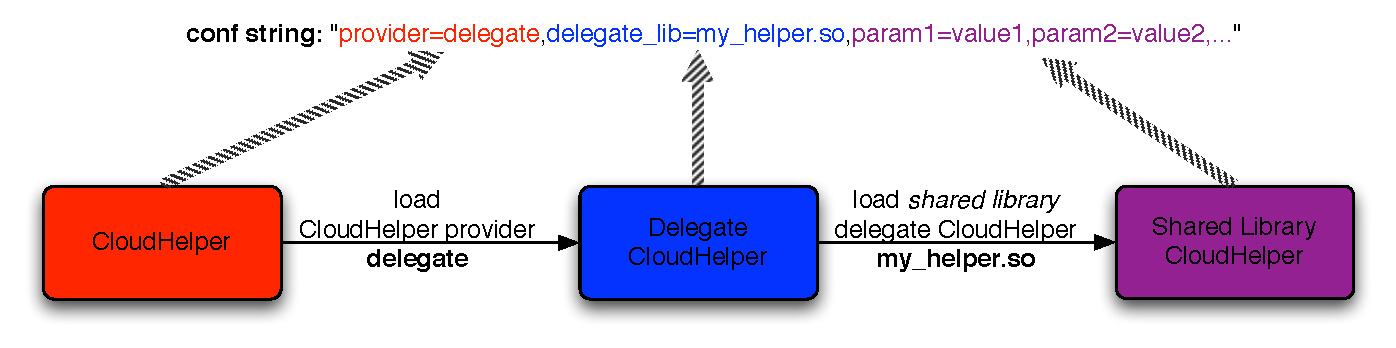
\includegraphics[width=\textwidth]{grapes-cloudhelper-lifecycle.pdf}
  \caption{\cloudhelper initialization diagram.}
  \label{fig:grapes-cloudhelper-lifecycle}
\end{figure}

\begin{table}[H]
  \centering
  \begin{tabular}{|l|l|}
  \hline
  Parameter & Meaning \\
  \hline
  \hline
  $mysql\_host$ & Hostname of the \textit{MySQL} database server \\
  $mysql\_user$ & \textit{MySQL} username \\
  $mysql\_pass$ & \textit{MySQL} password \\
  $mysql\_db$ & name of the database to use as cloud \\
  $mysql\_table$ & name of the table to use as bucket \\
  \hline
  \end{tabular}
  \caption{Provider specific parameters for \textit{MySQL} delegate helper.}
  \label{tbl:grapes-cloudhelper-mysql}
\end{table}

\begin{table}[H]
  \centering
  \begin{tabular}{|l|l|}
  \hline
  Parameter & Meaning \\
  \hline
  \hline
  $s3\_access\_key$ & \textit{Amazon} access key id \\
  $s3\_secret\_key$ & \textit{Amazon} secret access key \\
  $s3\_bucket\_name$ & name of the bucket to operate on \\
  $s3\_protocol$ & protocol used for communications. (\emph{http}  or
  \emph{https}) \\
  \hline
  \end{tabular}
  \caption{Provider specific parameters for \textit{Amazon S3} delegate helper.}
  \label{tbl:grapes-cloudhelper-libs3}
\end{table}

\section{\cloudcast \peersampling protocol}
The \cloudcast \peersampling protocol implementation is fully
integrated in the \grapes \textit{Peer Sampling} \api and doesn't
require any specific action to be taken by the final application in
order to work. The source code follows the algorithm showed in
section~\ref{sec:cloudcast-additions} and thus will not be reported
here as it does not give any substantial contribute. Instead this
section will give some insight on the configuration and usage of the
protocol.

Table \ref{tbl:grapes-cloudcast-parameters} reports the supported
configuration parameters along with their meaning and their default
value. As can be seen none of them is required to obtain a fully
functional instance, however by default the recovery mechanism
discussed in section~\ref{sec:cloudcast-additions} is not enabled
and this may cause some problem as it will be shown later on.

\begin{table}[H]
  \hspace{-20pt}
  \begin{tabular}{|p{0.27\textwidth}|p{0.63\textwidth}| c |}
  \hline
  Parameter & Meaning & Default\\
  \hline
  \hline
  $period$ & period of the active cycle (\deltacyclon) in
  seconds & 10s \\
  $cache\_size$ & size of the local \view ($c$) & 20 \\
  $sent\_entries$ & size of the partial \view ($g$) & 5\\
  $view\_key$ & key used to host the \cloud \view & ``view'' \\
  $max\_silence$ & max number of global cycle without \cloud
  contact (\maxsilence $*$ \deltacyclon) & 0 \\
  $cloud\_respawn\_prob$ & probability of creating a new \cloud
  \descriptor when silence threshold is reached (\spawnprob) defined
  in [0,1] & 0\\
  \hline
  \end{tabular}
  \caption{\cloudcast \peersampling protocol implementation
    parameters. Parenthesis enclosed values represent the
    corresponding entities in the algorithm.}
  \label{tbl:grapes-cloudcast-parameters}
\end{table}

Figure \ref{lst:grapes-example-app} shows a minimal application which
successfully takes part in a \cloudcast \peersampling protocol
instance. The differences with respect to a standard \grapes
application which exploits the \emph{Peer Sampling} module are limited
but substantial. First and most notably the \cloudhelper must be
loaded and configured, this is done in line 2 and 13-15 by including
the \textit{cloud\_helper.h} header file and by creating a new
\textit{context}. In the example the actual \cloud support is offered
by the fictional \textit{my\_helper.so} library.
The next noteworthy operation can be seen in line 16: here the actual
\peersampling protocol is loaded by specifying the value
\textit{cloudcast} for the \textit{protocol} parameter. A custom value
for the \textit{cache\_size} parameter is specified to give a better
understanding of the configuration mechanism.

The only remaining difference with respect to a standard application
regards the handling of incoming
data. Indeed given that \grapes design delegate the receiving of data
to the application, this is now responsible to read incoming messages
from both the peers and the \cloud. To help with this task, two
commodity function were developed and are exposed via the
\textit{cloud\_helper\_utils.h} header file: \textit{wait4any\_thread} and
\textit{wait4any\_polling}. The former concurrently invokes the wait
functions of the \textit{Network Helper} and \cloudhelper modules,
while the second uses a polling scheme to avoid the added dependencies
that the \textit{thread} abstraction layer takes with itself. The
first variant of this functionality can be seen in action in line 25.

These are all the information needed to successfully use the
\cloudcast \peersampling protocol implemented in \grapes in a C
application. A more exhaustive documentation of the functions discussed
in this section (and many other) is provided within the headers file
distributed alongside the source code.

\begin{figure}[H]
  \centering
  \lstinputlisting[language=C,basicstyle=\footnotesize,numberstyle=\footnotesize,numbers=left,frame=single]{code/grapes-example.c}
  \caption{Skeleton of a simple application using the \cloudcast
    \peersampling protocol.}
  \label{lst:grapes-example-app}
\end{figure}

\section{Building and deployment}
The modification to the toolkit were developed with the
support of \grapes's authors and are in the process of being merged
into the main codebase. The actual code developed during the course of
this work is available via \github~\cite{GRAPES-repo}: the tag
\thesistag point to the \emph{HEAD} revision at the moment of this
writing.

The building process is unaltered and follows the conventions
established by \grapes: to generate the main library just type ``\make''. This
will result in the creation of a \emph{static} library named
``\textit{libgrapes.a}'' containing all of the functionality apart
from the \cloudhelper delegate implementations. These must be compiled
separately by entering in the \texttt{src/CloudSupport/} directory and
typing ``\make delegate\_helpers``. Such command will generates a
separate \textit{shared} library for each available delegate
helper. The \texttt{PLATFORM} variable can be used to select the
desired library format: at the current state supported values are
\textit{unix} and \textit{darwin}.
Note that before being able to build the delegate helpers, the
\emph{libs3} and \emph{MySQL Connector/C} libraries must be
installed and configured.

\section{Java bindings}
As was mentioned in the introduction, the final goal of this work is
the creation of a general framework written in \emph{Java}. This poses
the problem of how exploit the modified \grapes toolkit from a
\emph{Java} application. In order to solve such problem a simple
library was developed to provide the bindings needed bindings. This
library is called \jgrapes.

It's designed in such a way to offer a one-to-one mapping with respect
to the \grapes's modules: the available classes are
\texttt{NetworkHelper}, \texttt{CloudHelper} and
\texttt{PeerSampler}. Each one of these exposes methods mapping the
\api of the respective \grapes module. The only design difference is
represented by the \texttt{JGrapes} class which function as a
\textit{single point of entry}: it takes care of loading the native
library and perform the required initialization action, furthermore it
provides simple function to allocate new instances of the main
components.

The usage of the library should be evident to anyone who is already
familiar with \grapes, in any case the package \emph{test} contains
a simple working application which shows the common usage.

Again the library is available via \github~\cite{jGRAPES-repo}, with
the \emph{HEAD} revision at the time of this writing tagged with
\thesistag.

The building process if fully automated and make usage of \emph{ant}
for the \emph{Java} portion and \make for the native components. The
first step is to update the \grapes distribution which will be used by
the library.
This is done by typing the command: \\
``\texttt{ant update-grapes
  -DGRAPES\_DIR=/path/to/grapes/distribution}''.

As a result both the
main \grapes library and the \cloudhelper delegate libraries will be
compiled and prepared to be used with \jgrapes. The same consideration
on the availability of the library dependencies made for
\grapes applies here so, in case of error during this phase, check
your environment.

The second step is the compilation of the \emph{Java} library
itself. This is done by invoking the target \texttt{dist} of the
\emph{ant} build file. During this second phase a series of things
happen: the final \emph{shared} library is created, the \textit{Java}
toolkit is compiled and packaged and in conclusion all the file
required to use the functionalities are placed in the \texttt{dist}
directory.
Since \jgrapes makes extensive use of \emph{JNI}~\cite{JNIGuide}, for this
phase to complete successfully, the location of \emph{JNI}'s header
files must be configured in the environment.

\section{Evaluation}
In conclusion of this chapter we would like to shows some tangible
result which shows how the real implementation perform compared with
the simulated one.
The experiments were performed via a \emph{Java} application
(available in the repository of \jgrapes) using the same configuration
parameter adopted by the corresponding simulations. When possible the
exact same setting used in the simulation was replicated, but some
specific experiment were impossible to fully reproduce due to limited
time (each simulated day requires one real day) and computational
resources.

\begin{figure}[h!]
  \centering
  \subfloat[][\emph{Cloud} in-degree]{
    \hspace{-70pt}
    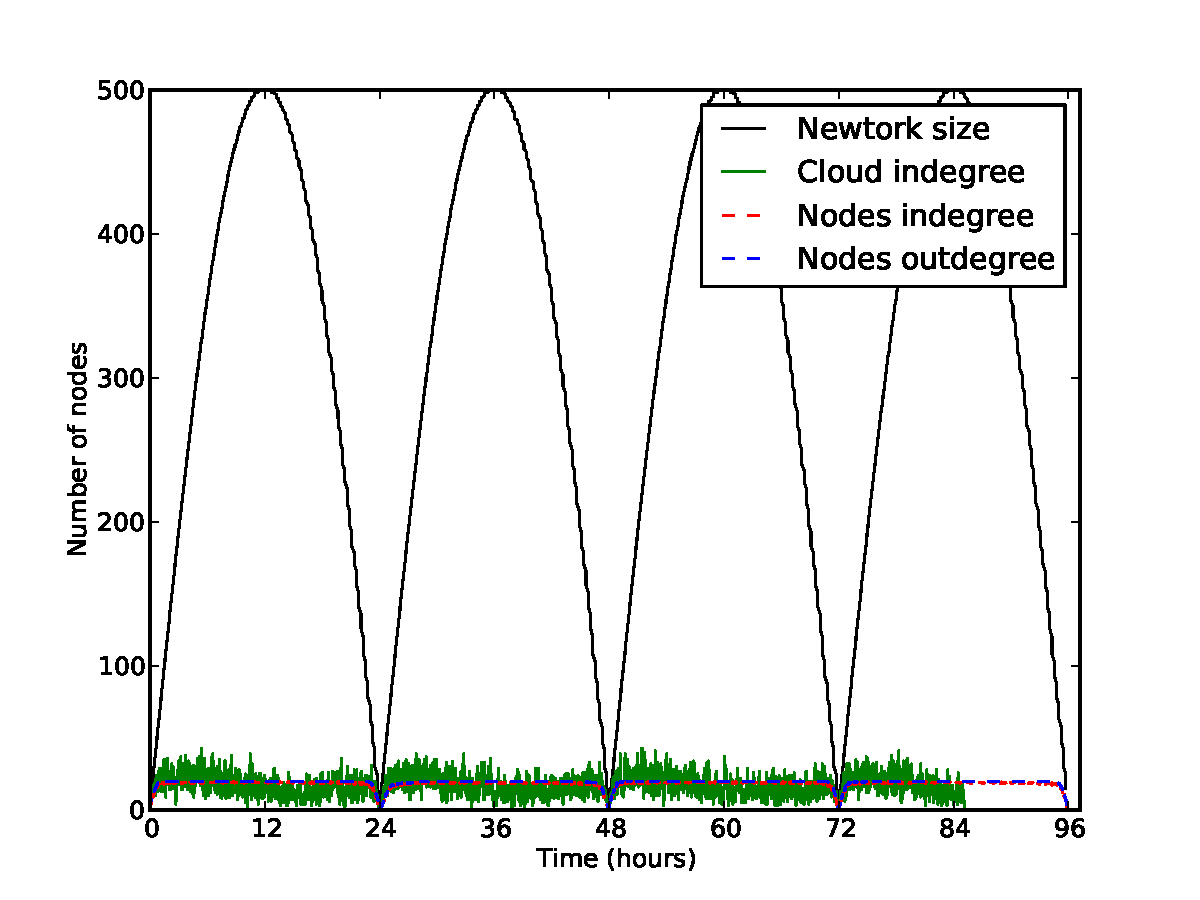
\includegraphics[width=240pt]{cloudcast-dynamic-indegree-4gg-0cloud.pdf}
    \label{fig:cloudcast-dynamic-indegree-original}
  }
  \subfloat[][\emph{Cloud} contacts]{
    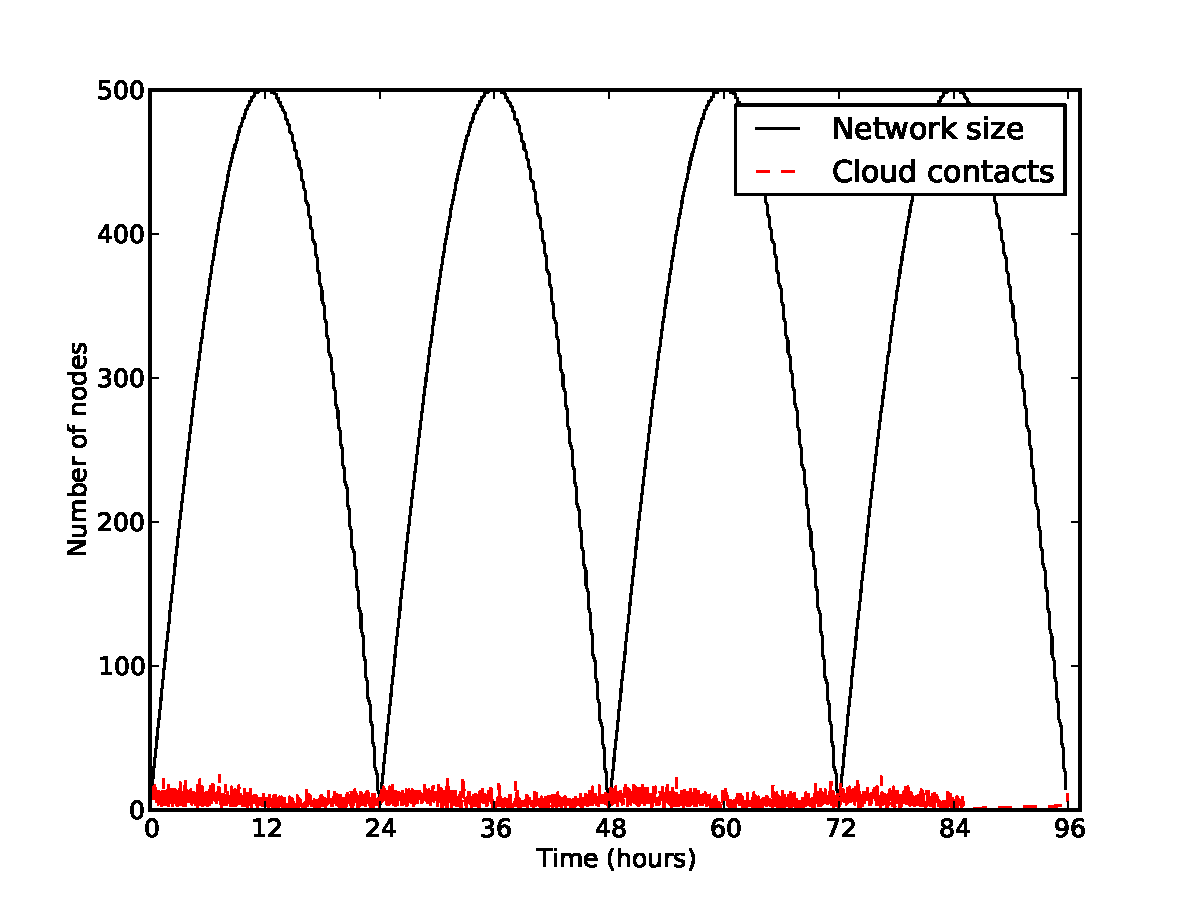
\includegraphics[width=240pt]{cloudcast-dynamic-load-4gg-0cloud.pdf}
    \label{fig:cloudcast-dynamic-load-original}
  }
  \caption{Behavior of the original \peersampling protocol}
  \label{fig:cloudcast-dynamic-original}
\end{figure}


The first result, shown in figure~\ref{fig:cloudcast-dynamic-original}
and matching figure~\ref{fig:cloudcast-sim-oscillating-indegree},
exhibit the behavior of the system when using the original protocol
without the recovery mechanism. As can be seen the protocol works as
expected for the first $3$ days, maintaining the desired \cloud
in-degree and contact rate, but as soon as the network start its
descending phase on day $4$, all the \cloud entries are lost and the
cloud is for all intent and purposes cut off the system. During the
analysis of \cloudcast it was already discussed how such a scenario
may happens, in this case however another factor plays an important
role. The way the \emph{Peer Set} module is currently implemented in
\grapes and the strategy used to maintain multiple \cloud entries by
the modified \cyclon make so that two \cloud \descriptor may be
collapsed into a single one during \view exchange. Such problem
requires a fairly extensive modification of the way \grapes handles
\descriptors to be fixed, so it wasn't feasible to fix it right
away. Anyway on its own the bug does not influences the behavior of
the protocol as it's demonstrated by the first $3$ days of execution
and by extensive tests performed on fixed size networks.

\begin{figure}[h!]
  \centering
  \subfloat[][\emph{Cloud} in-degree]{
    \hspace{-70pt}
    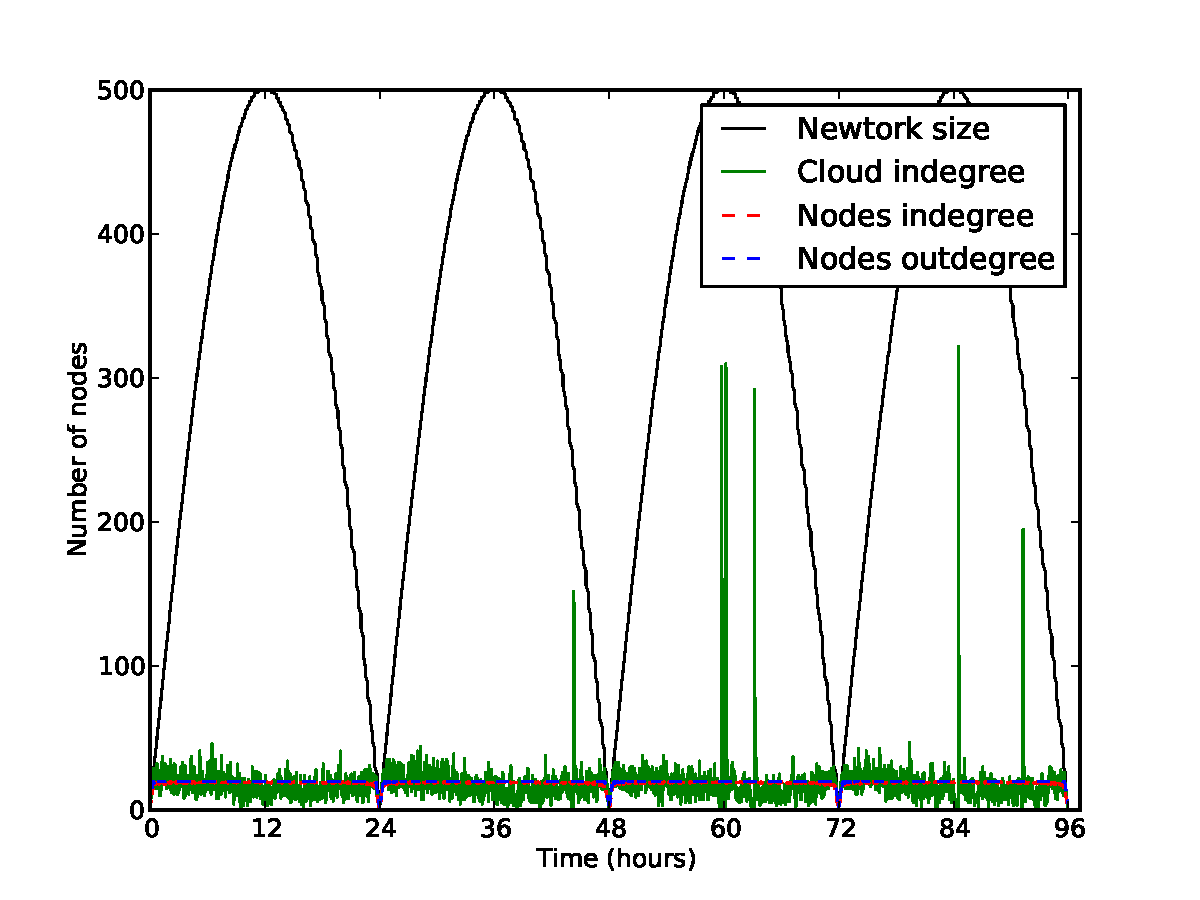
\includegraphics[width=240pt]{cloudcast-dynamic-indegree-4gg.pdf}
    \label{fig:cloudcast-dynamic-indegree-additions}
  }
  \subfloat[][\emph{Cloud} contacts]{
    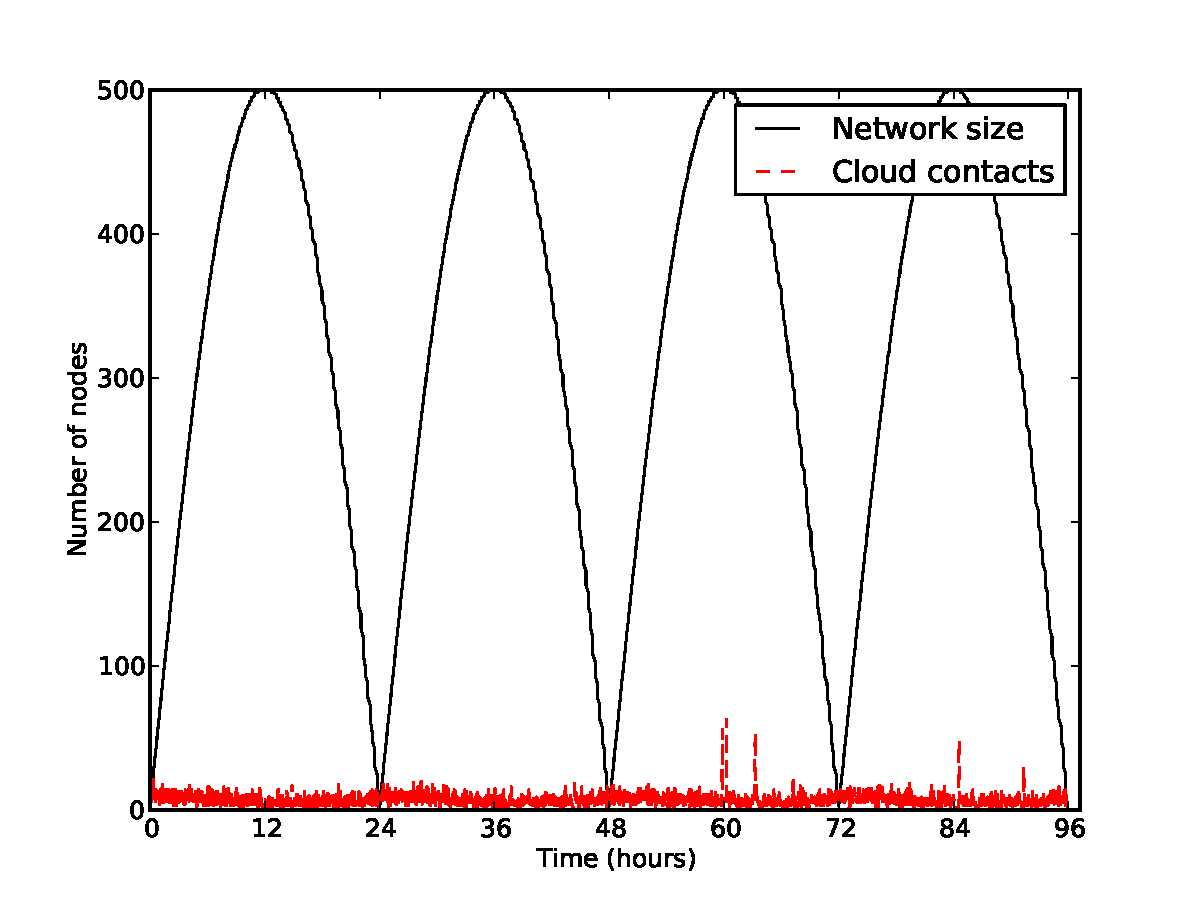
\includegraphics[width=240pt]{cloudcast-dynamic-load-4gg.pdf}
    \label{fig:cloudcast-dynamic-load-additions}
  }
  \caption{Behavior of the modified \peersampling protocol}
  \label{fig:cloudcast-dynamic-additions}
\end{figure}


Figure~\ref{fig:cloudcast-dynamic-additions} shows the same experiment
performed using the modified \cloudcast protocol. The additional
parameter used to perform these tests are:
\begin{itemize}
  \item $max\_silence$: 30 cycles
  \item $cloud\_respawn\_prob$: 0.2
\end{itemize}

The first thing that can be noted observing the
plot~\ref{fig:cloudcast-dynamic-indegree-additions} is the presence of
high peak of \cloud \descriptors. This is the effect of the recovery
mechanism in action. As can be seen the peaks are reabsorbed quickly
and as shows plot~\ref{fig:cloudcast-dynamic-load-additions} the
impact on the \cloud contact rate is fairly limited and shouldn't
impact much on the aggregated daily contacts.

\begin{figure}[h!]
  \centering
  \subfloat[][``clean'' run]{
    \hspace{-70pt}
    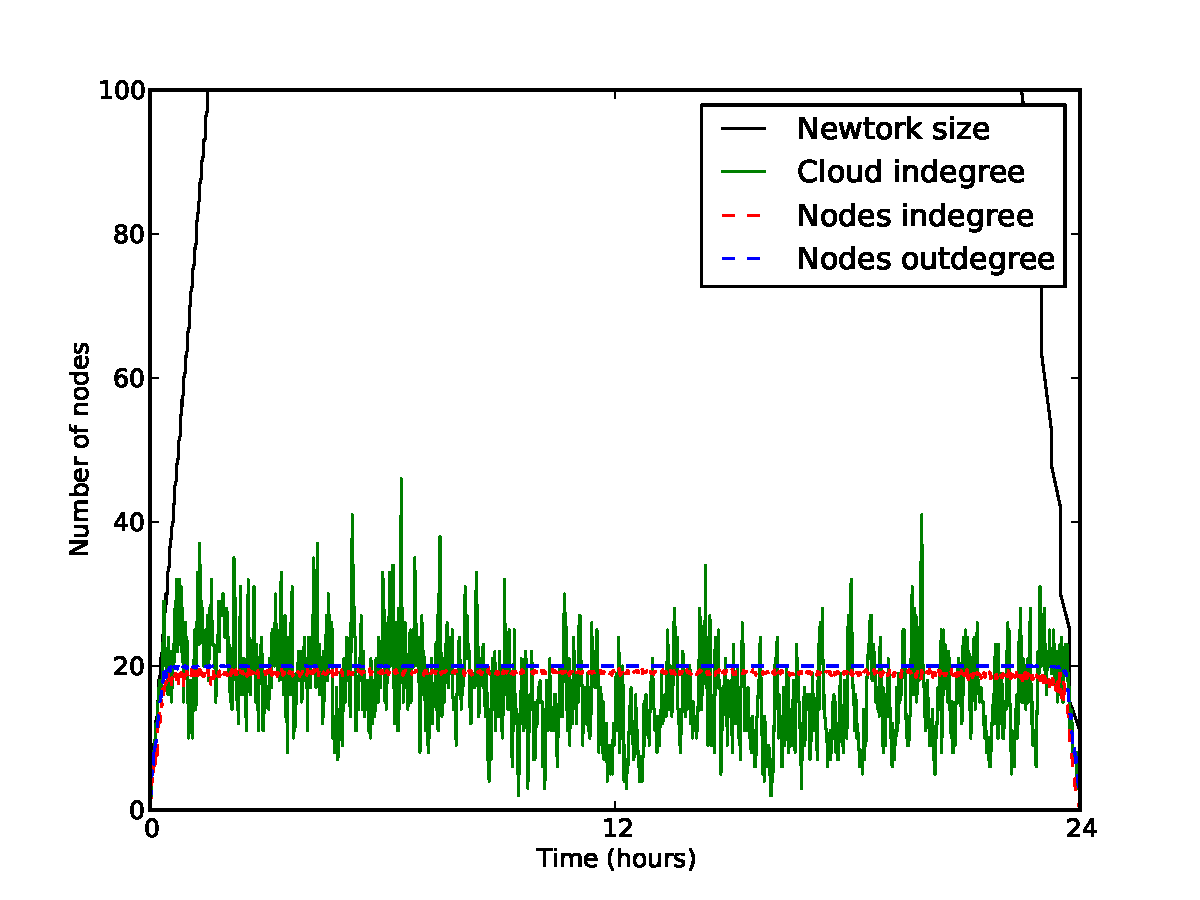
\includegraphics[width=240pt]{cloudcast-dynamic-indegree-4gg-detail-norecovery.pdf}
    \label{fig:cloudcast-dynamic-indegree-additions-detail-norecovery}
  }
  \subfloat[][Recovery mechanism in action]{
    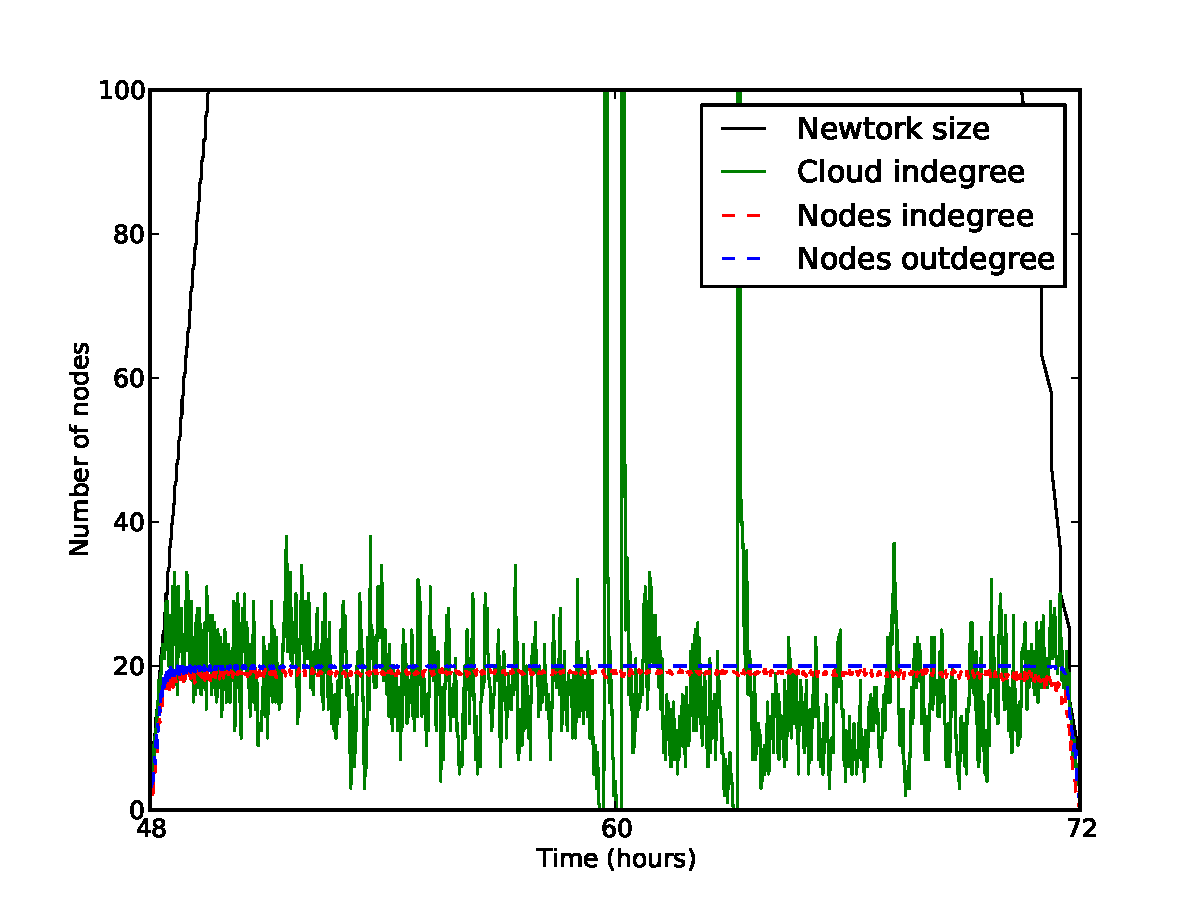
\includegraphics[width=240pt]{cloudcast-dynamic-indegree-4gg-detail-recovery.pdf}
    \label{fig:cloudcast-dynamic-indegree-additions-detail-recovery}
  }
  \caption{Zoomed in plots comparing the effects of the recovery
    mechanism on the \cloud in-degree}
  \label{fig:cloudcast-dynamic-indegree-additions-detail}
\end{figure}


Figure~\ref{fig:cloudcast-dynamic-indegree-additions-detail} shows a
comparison between ``clean'' day of execution and another in which the
recovery mechanism fired multiple times. First of all it easy to see
how the overall performance is similar in both plot: the average
number of \cloud \descriptors tend to approximate the desired value in
both plot.
More interesting is the behavior exhibited by the recovery mechanism:
around the $60^{th}$ hour of execution it is fired 2 times in a close
succession. Such a chain of events don't happen often, but it shows
how the recovery mechanism and the \cloud rate adaptive scheme works
on the two opposite fronts: the former notice that too much time is
passed since the last global \cloud contact and respond by creating a
number of \cloud \descriptors randomly distributed in the network. The
latter react to the suddenly increase in contact by removing
them.
This two competing force alongside the usual descending phase of the
network and an unlucky succession of \view exchanges have the effect
of once more removing all the \cloud entries in the network.

Considering as the starting instant the moment in which the number of
\cloud \descriptors goes to $0$ for the fist time and as ending
instant the time in which the network stabilizes itself after the
second activation of the recovery mechanism, the total time taken by
this stalling phase is around one hour. In the meantime the protocol
still works without problems even though the target \cloud contact
rate is not respected.

\begin{figure}[h!]
  \centering
  \subfloat[][``clean'' run]{
    \hspace{-70pt}
    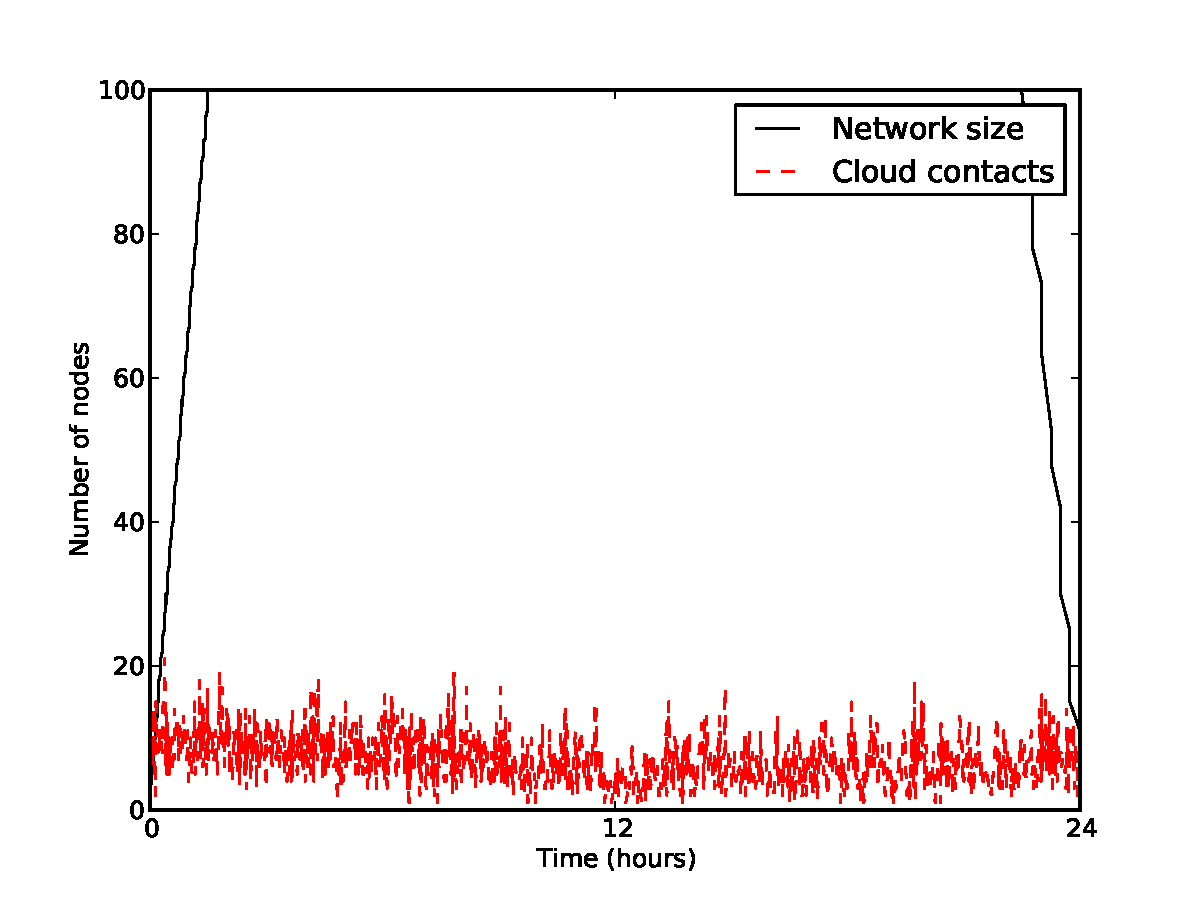
\includegraphics[width=240pt]{cloudcast-dynamic-load-4gg-detail-norecovery.pdf}
    \label{fig:cloudcast-dynamic-load-additions-detail-norecovery}
  }
  \subfloat[][Recovery mechanism in action]{
    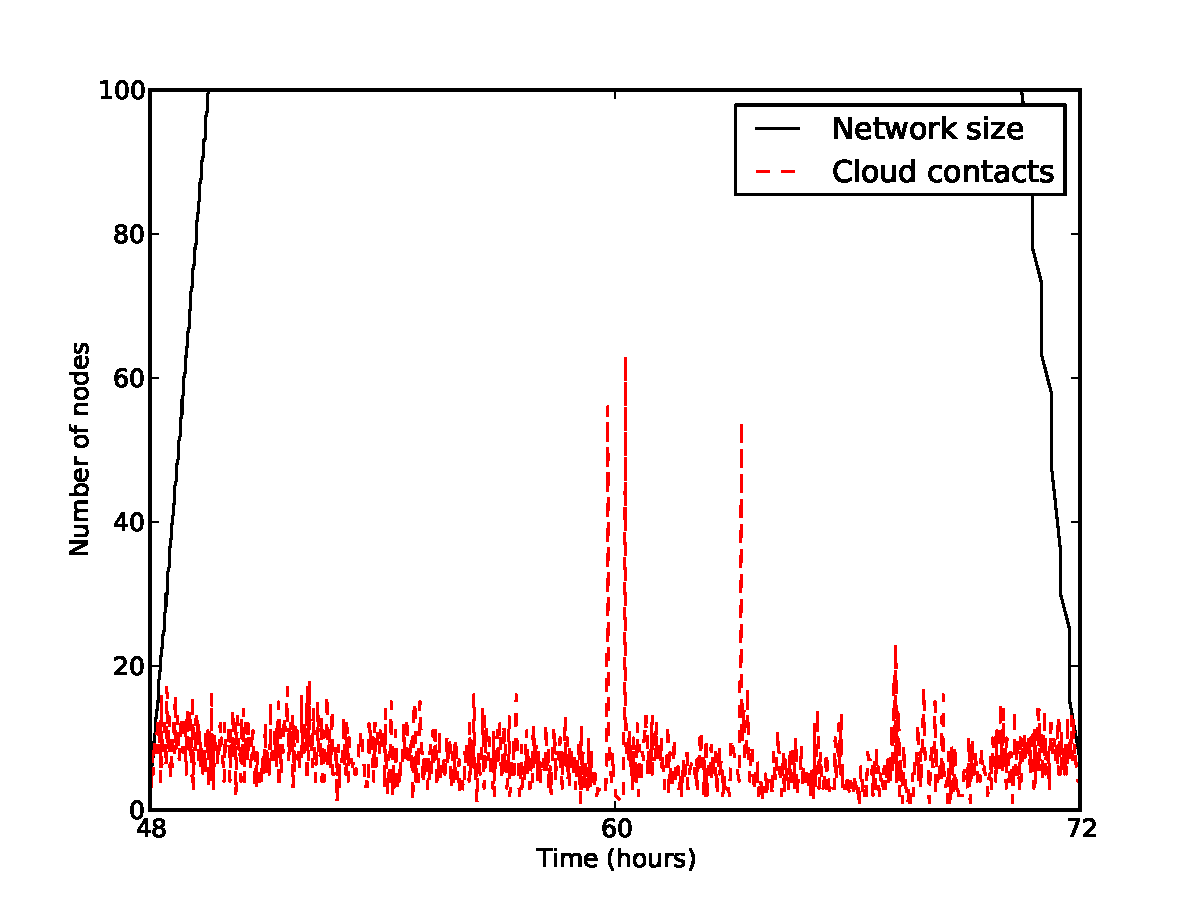
\includegraphics[width=240pt]{cloudcast-dynamic-load-4gg-detail-recovery.pdf}
    \label{fig:cloudcast-dynamic-load-additions-detail-recovery}
  }
  \caption{Detail of \cloud highlighting the effects of the recovery mechanism}
  \label{fig:cloudcast-dynamic-load-additions-detail}
\end{figure}

Figure~\ref{fig:cloudcast-dynamic-load-additions-detail} shows the
same two days from the point of view of the \cloud contact rate. In
these plot is more evident how limited is the influence of the
recovery mechanism: the peak are relatively small and they lasts for
limited amount of time.

The parameter used to configure the recovery mechanism was not
subjected to evaluation, they were selected so to be somewhat
realistic but without any deep consideration on the impact. Thus
by selecting them more carefully or even better by employing some
adaptive strategy the overall impact should sensibly decrease.

\begin{figure}[h!]
  \centering
  \subfloat[][Real implementation results]{
    \hspace{-70pt}
    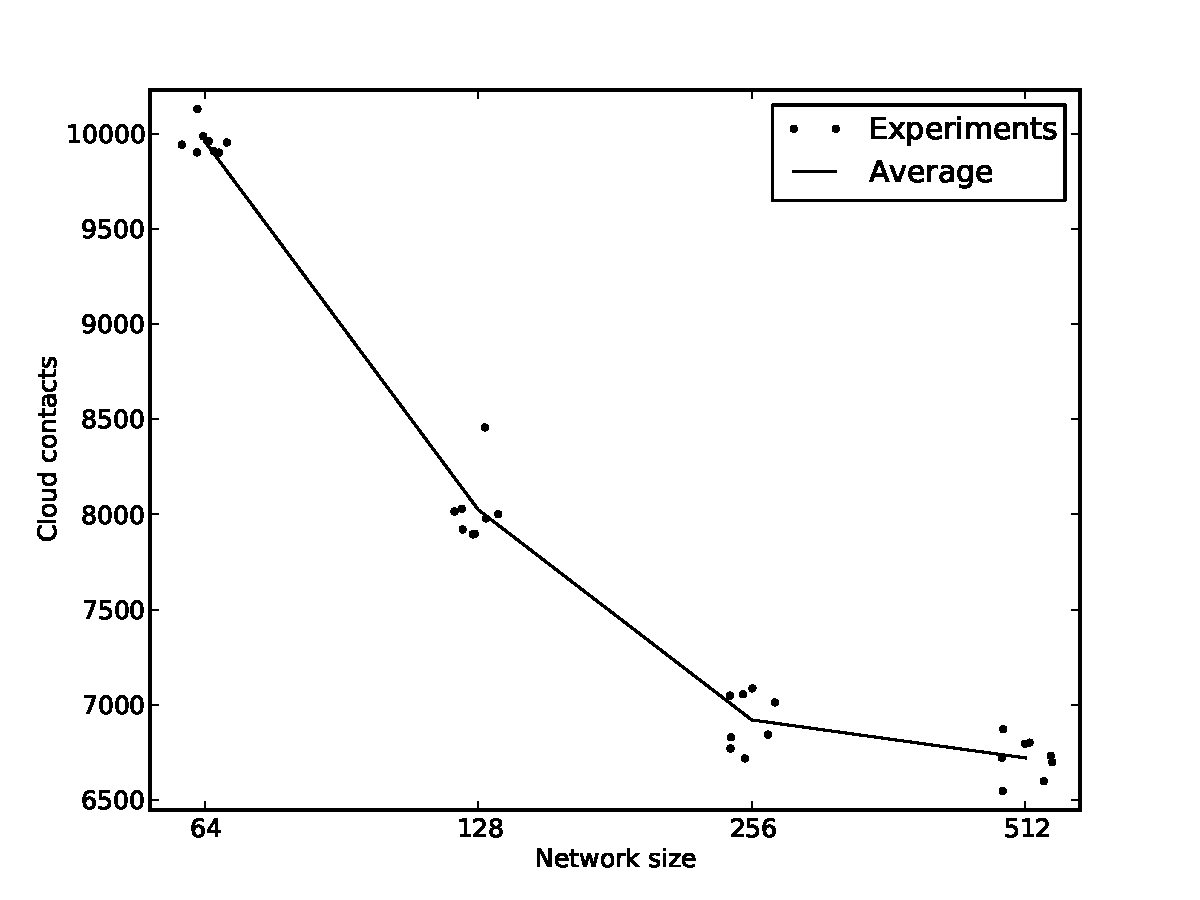
\includegraphics[width=240pt]{cloudcast-loads.pdf}
    \label{fig:cloudcast-loads}
  }
  \subfloat[][Simulated results]{
    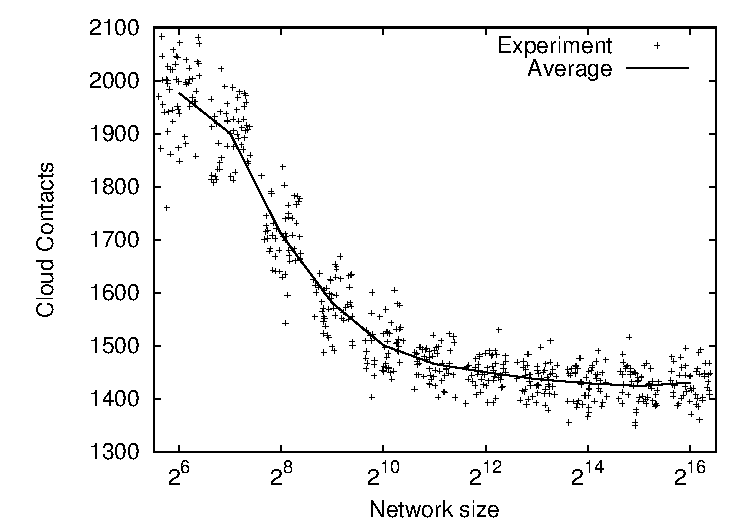
\includegraphics[width=240pt]{cloudcast-sim-loads.pdf}
    \label{fig:cloudcast-sim-loads-re}
  }
  \caption{Storage \cloud load for different network sizes.}
  \label{fig:cloudcast-loads-global}
\end{figure}

Figure~\ref{fig:cloudcast-loads-global} conclude the evaluation of the
implementations. The plot~\ref{fig:cloudcast-loads} show the \cloud
load obtained by the \grapes implementation for different network
size and match the plot in figure~\ref{fig:cloudcast-sim-loads} which
is repeated in plot~\ref{fig:cloudcast-sim-loads-re} for convenience.

Due to difference in the experiment setup and in the way data was
collected the values in the two plots are not directly comparable,
however is evident how they are proportional. In both the \cloud
contact rate is high for small networks and it tend to decrease as
more nodes are added.

The odd result obtained by the real implementation for a network size
of $1024 = 2^{10}$ is also the reason why we didn't provide samples for
denser network. The test were performed on a small number of shared
server. To simulate $1024$ nodes $4$ real machine were employed each
taking care of $256$ peers in the form of an equal number of
\emph{Java} threads. The excessive computational load posed on each
machine caused delays, missed messages and in the end resulted in the
bad performances of the protocol. Simulation with a higher number of
nodes weren't even able to run until completion.

\chapter{The CloudyPeer framework}
As is stated in the
introduction, \cloudypeer aims to be a general framework for building
\ptop application focused on data dissemination scenarios.
In particular the final goal of the project is to give developers the
ability to create such applications with the minimum amount of code as
possible, concentrating their effort in planning the logic of the
application instead of the underlying \ptop infrastructure.

This convenience however must not come at the price of
flexibility: often times the design of a \ptop application requires
tweaking at the lower level of the infrastructure; in these situations
a static and monolithic framework may represent an obstacle instead of
an help.
In this regards \cloudypeer must enable developers to extend its
functionality in an easy and integrated way without breaking the other
requirements.

Another important factor which has been considered during the
planning phase is that the performances of a \ptop application may
vary substantially by changing the specific protocol offering a
particular functionality, or by tuning its parameters. Often this
evaluation stage is performed in a simulated environment due to timing
constraints and ease of development. However simulations not always
reflect what happens when the same protocol is implanted in a real
scenario.
The \cloudypeer architecture has been explicitly designed to allow the change
of every single component by simply modifying a configuration
parameter thus allowing experimenting with different
combinations without the need to touch a single line of code.

The implementation is based on the \emph{Java} programming language and it's
compatible with version 1.5 or higher. The
choice of \emph{Java} is motivated by the fact that it provides a rich
\emph{standard library} and its object oriented nature makes it a
perfect candidate for designing an extensible framework. Furthermore
the existence of many commercial and open-source projects written in
\emph{Java} and concerning \ptop systems represent a valuable resource
in term of code reuse.
\ \\
In the following sections will be analyzed the architecture of
\cloudypeer by describing it's major components and their interactions.
Furthermore will be described the various module's
built-in implementations and the means offered to developers to extend
the framework itself.
In conclusion a ``toy'' application will be shown with the intent of
demonstrating the simplicity and the convenience offered by
\cloudypeer.

As for the previous chapter the notation rules adopted in the
following portion of the chapter are:
\begin{itemize}
  \item serif font for files and directories, i.e. \textsf{ExampleFile.java},
    \textsf{./example\_directory/}
  \item italics font with capitalized initials for module names,
    i.e. \textit{Example Module)}
 \item typewriter font for class names, i.e. \texttt{ExampleClass}
  \item italics font followed by parenthesis for methods
    i.e. \textit{exampleMethod()}
  \item standard UML notation for diagrams
\end{itemize}

\section{Architecture}
Figure \ref{fig:cloudypeer-architecture} shows an overview of the
architecture of \cloudypeer illustrating the principal components and
the way they are related one another.

\begin{figure}[h!]
  \centering
  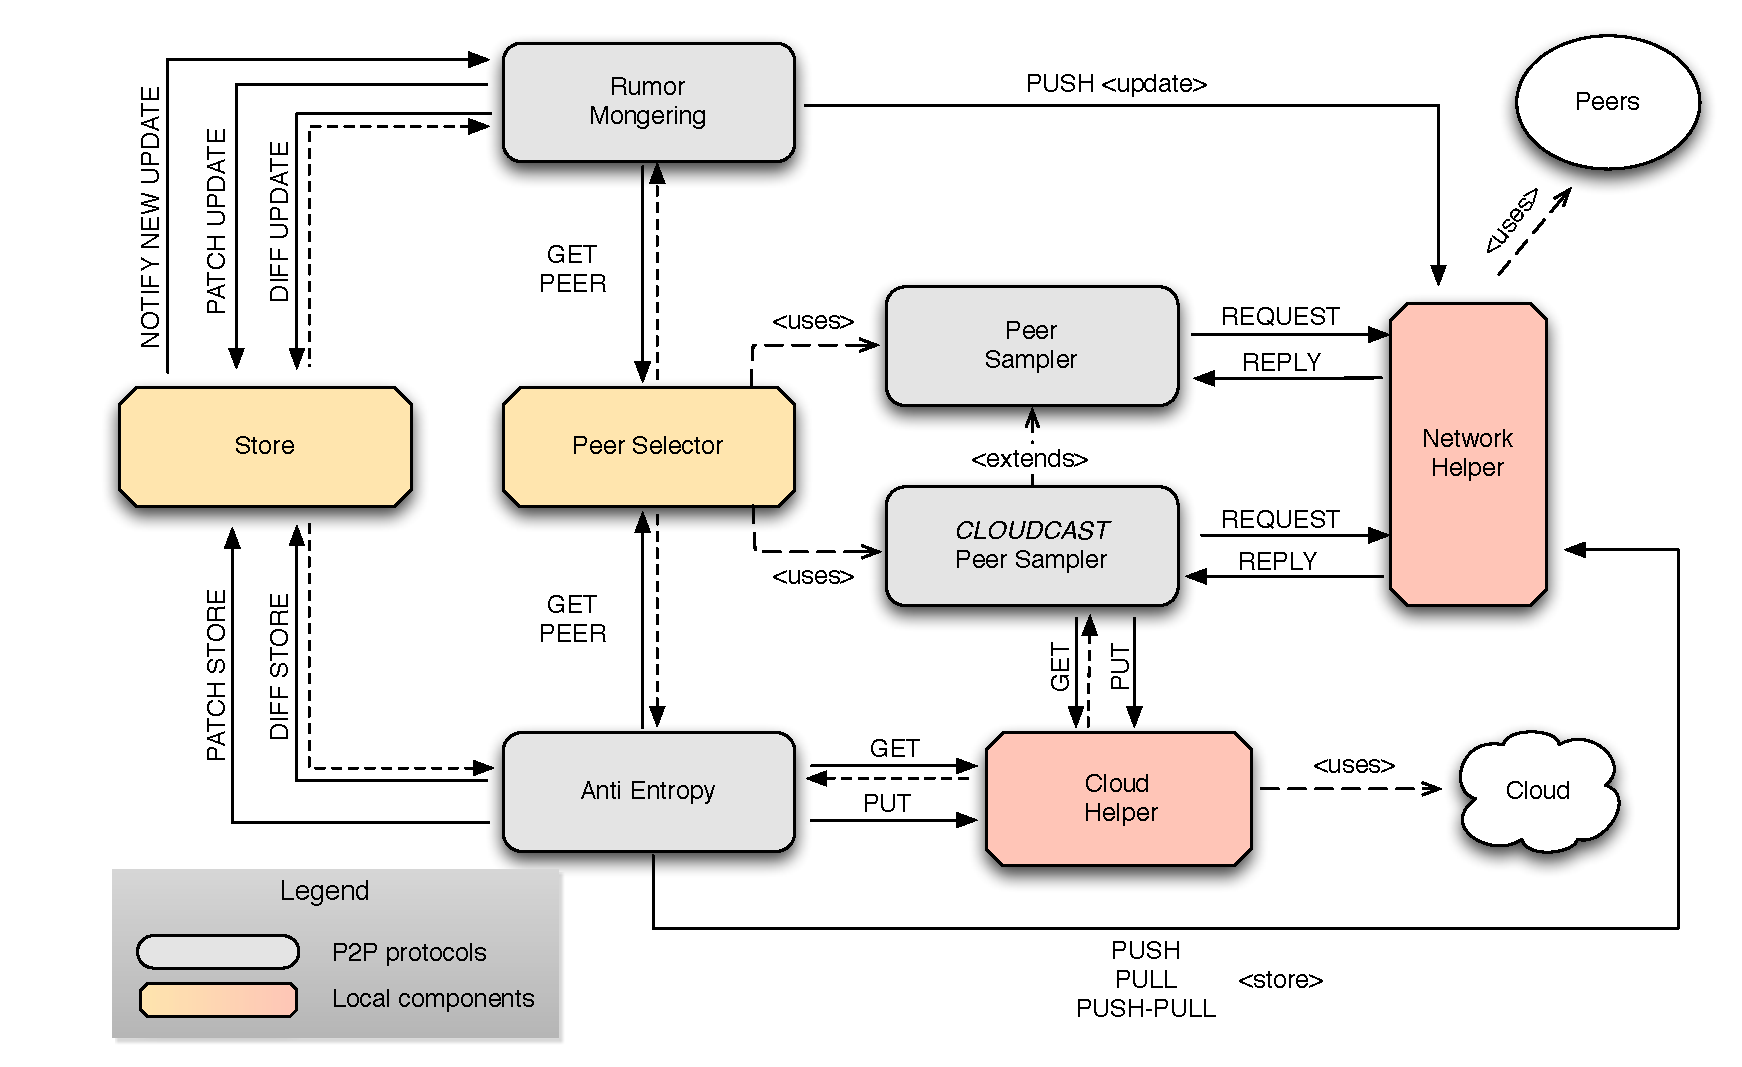
\includegraphics[width=\textwidth]{cloudypeer-architecture.pdf}
  \caption{Architectural overview of \cloudypeer}
  \label{fig:cloudypeer-architecture}
\end{figure}

As can be seen, the \peersampling protocols hold a central role in the
infrastructure and are divided in two categories: the first represents
classic protocols such as \cyclon; the second extends the former and
embodies the \peersampling protocol of \cloudcast.

Samples of the network's partial \view\ are offered to higher level
protocols via a \peerselector. This is a local module which does not
directly interact with the \ptop network but it just implements the logic
used by the application to select peers. This abstraction gives the
opportunity to application's developers to implement complex selection
strategies, possibly involving multiple \peersampling instances of
different kind. A simple implementation performing a random
selection with customizable filters is provided within the framework
and should be sufficient for most of the simpler scenarios.

The \peerselector itself is used by all the algorithms which are
based on the interaction between pairs of peers. At the current stage
the only components of such kind are the two variants of \epidemic
broadcast, but more can be easily added.

The function executed by these two protocols necessarily requires
access to the application data. However such a direct dependency
does not fit with
the generality requirement of the framework. For this reason the
\store abstraction layer has been added: this component provides a general
\api for accessing and managing the application data which other
modules can use to modify the application state.

Application designers must create their own \store implementation
reflecting their storage model. To simplify this task the framework
provides a built-in implementation which takes care of most of the
operation needed to fulfill the \api specifications.

The modules which conclude this architecture overview are the
\cloudhelper and \networkhelper: similarly as what has been discussed for
\grapes, these two elements provide an abstraction layer which hides
the details of the actual implementations making it possible
to easily switch \cloud provider or networking technique.

\ \\
The following sections will cover the details of the aforementioned
modules by providing a more in depth description of the \api they
offer and by giving some insight on the way to extend them.

\section{Basic components}
Before starting the description about the specific modules, let's look
at figure~\ref{fig:cloudypeer-basic-relations} where are shown the
basic components which are used by the rest of the \cloudypeer
infrastructure.

\begin{figure}[h!]
  \centering
  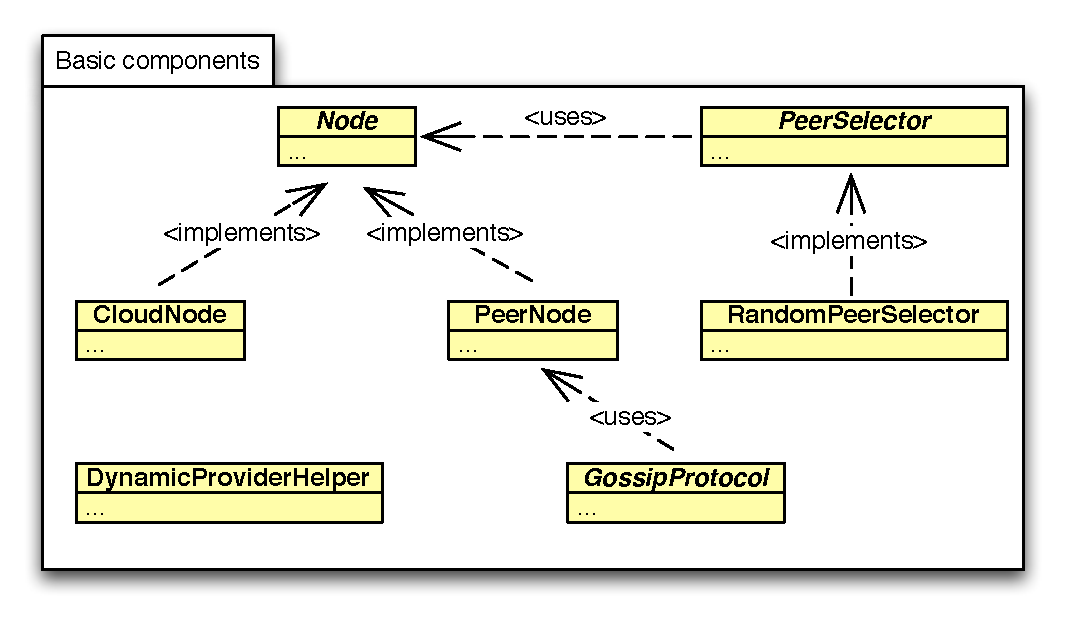
\includegraphics[width=\textwidth]{cloudypeer-basic-relations.pdf}
  \caption{\cloudypeer basic components}
  \label{fig:cloudypeer-basic-relations}
\end{figure}

Most of the classes role should be already clear at this point:
\texttt{Node} and its two implementation are used to model
node \descriptors and provide basic addressing information while
\texttt{PeerSelector} defines a standard way to express
peer selection strategies, of which \texttt{RandomPeerSelector} is a
simple example.

The remaining two classes instead deserve more attention.

\noindent\texttt{DynamicProviderHelper} is an utility component which
provides the infrastructure needed to dynamically load object's
implementations. It performs hierarchical parsing of provider's
configurations file enabling for end-user overwriting of the
preferences and handles the instantiation of the correct
implementation via name mappings. Since its presence results completely
transparent to users of \cloudypeer it will not be proposed a detailed
description of its working. Developers interested in extending the
framework with new protocols may refer to the \javadoc of the project
for further information on how to exploit the dynamic loading procedures.

\begin{figure}[h!]
  \centering
  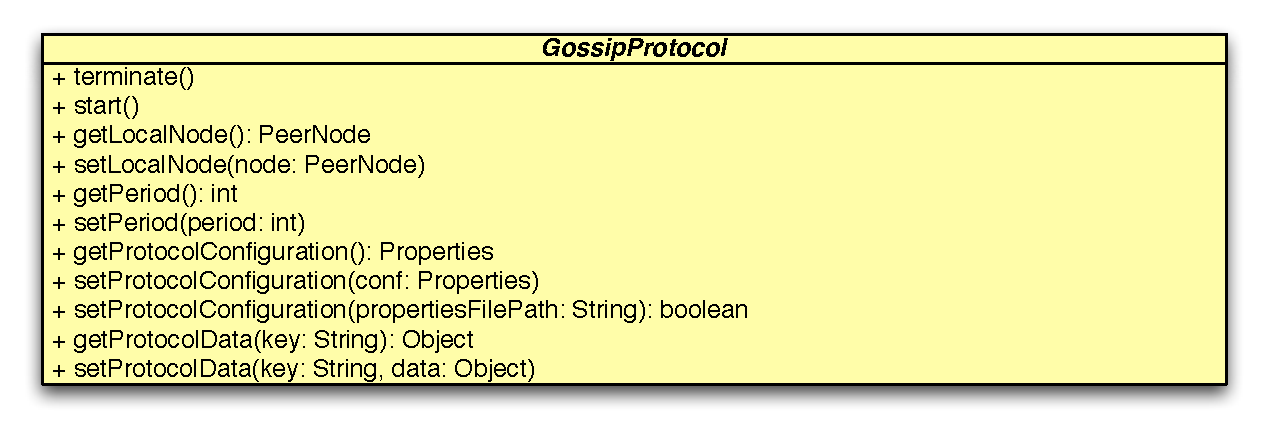
\includegraphics[width=\textwidth]{cloudypeer-basic-gossipprotocol-classdiagram.pdf}
  \caption{\texttt{GossipProtocol} public \api}
  \label{fig:cloudypeer-gossipprotocol-class}
\end{figure}

The last class composing the basic infrastructure is
\texttt{GossipProtocol}. A diagram describing this abstract class is
provided in figure~\ref{fig:cloudypeer-gossipprotocol-class}. This
component defines the skeleton of a \gossip protocol: it provides
standard means to start and stop the execution, configures the common
properties and furthermore it offers support for opaque parameters
and resources. Such features represent the public \api and
only reflect part of the offered functionalities: indeed
\texttt{GossipProtocol} implements many other common procedure aimed at
simplifying the thread management and the overall lifecycle of the
implementation.

\section{\networkhelper}
The \networkhelper module mission is to provide a simple abstraction
layer to the actual networking implementation. Its services are
available to any class wanting to use them, however it's usage is not
required to build a protocol in \cloudypeer. It's design is somewhat
inspired to the relative component of \grapes, but with some
additional features.

\begin{figure}[h!]
  \centering
  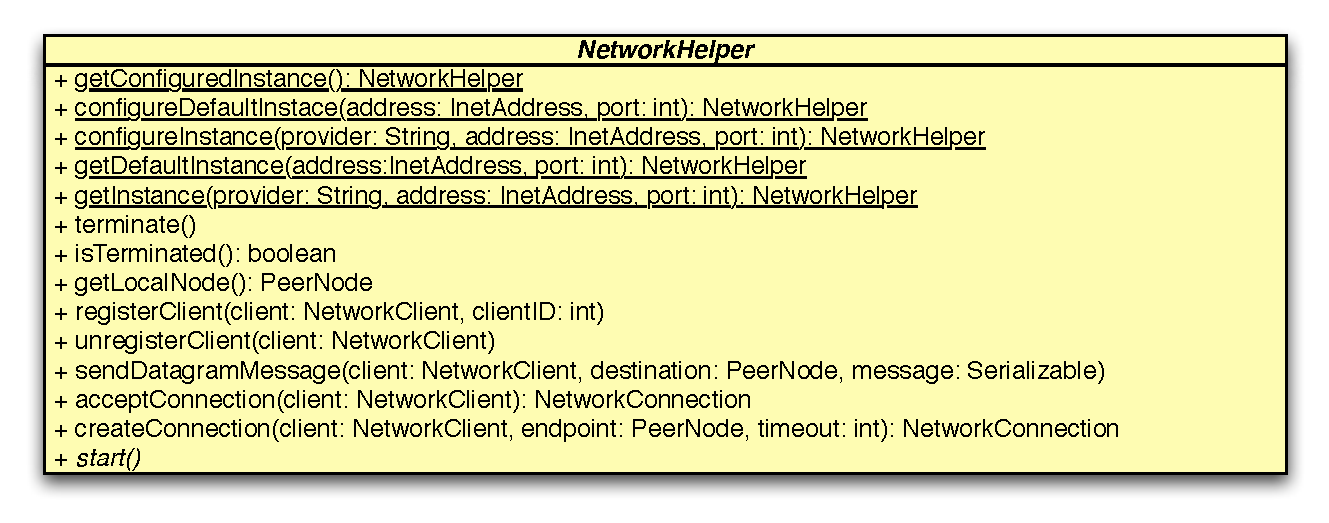
\includegraphics[width=\textwidth]{cloudypeer-networkhelper-classdiagram.pdf}
  \caption{\texttt{NetworkHelper} public \api}
  \label{fig:cloudypeer-nethelper-class}
\end{figure}

As can be seen by looking at the public \api shown in
figure~\ref{fig:cloudypeer-nethelper-class}, beyond datagram messages
\cloudypeer's \networkhelper offers support for connection oriented
transport protocols. The rationale of this choice resides in the fact
that some \ptop protocols require the exchange of a series of messages
to complete a cycle. Even though such requirement may be efficiently
achieved only by using datagram messages, the resulting code complexity is
substantial: by delegating this task to the \networkhelper, protocols
implementation can be much simpler. Even better, this strategy allow
for far more effective code reusage: custom connection schemes can be
implemented as a \networkhelper object and made available to
all \cloudypeer component by simply changing a configuration parameter.

\begin{figure}[h!]
  \centering
  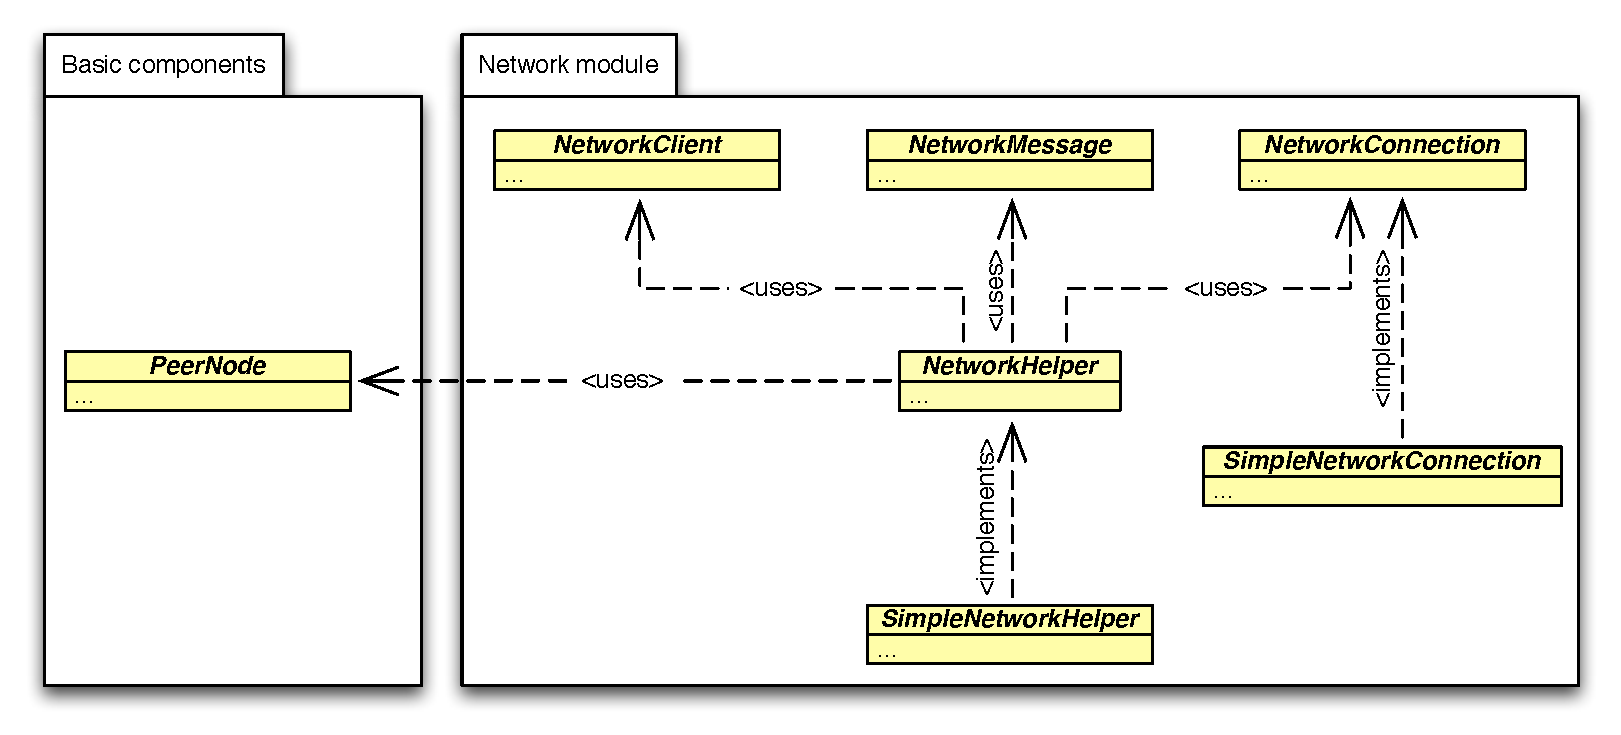
\includegraphics[width=\textwidth]{cloudypeer-networkhelper-relations.pdf}
  \caption{Relations between classes of the \networkhelper module}
  \label{fig:cloudypeer-nethelper-relations}
\end{figure}

A \networkhelper instance can be initialized by calling either the
\textit{getDefaultInstance} or \textit{getInstance} methods. The former
will load the default implementation as specified in the bundled
configuration file. The latter allows the caller to specify the
implementation to use. Another way to create a \networkhelper instance
is to ``configure'' it via the \textit{configureDefaultInstance} or
\textit{configureInstance} methods. In this way the newly created
instance will be stored and can be the recovered calling the
\textit{getConfiguredInstance} method.

Before a class is allowed to exploit a \networkhelper instance it must
implement the \texttt{NetworkClient} interface and
``register'' itself by calling \textit{registerClient}. The
registration phase maps the actual client instance to a specified
identifier. At this point the class can send datagram messages or
initiate connections to its remote counterparts. This means that a
\texttt{NetworkClient} can communicate only with remote
\texttt{NetwotkClient} instances sharing the same identifier.

\ \\
At the current stage only one \networkhelper implementation is
distributed with the framework: \texttt{SimpleNetworkHelper}. This class
relays on \emph{Java}'s network stack and exploits threads to allow
concurrent connections. In particular connection oriented
communication is achieved via \texttt{TCP} connection.
Another implementation, which hasn't been completed due to time
constraints, is based upon \grapes's \networkhelper thus inheriting
the \emph{NAT  traversal} supports.

\section{\cloudhelper}
The support for the \cloud storage service is offered via the
\cloudhelper module. Figure~\ref{fig:cloudypeer-cloudhelper-relations}
shows the components belonging to the module and their relations.
The central component of this module is \texttt{StorageCloud} which
implements the actual \cloud interaction logic. The offered \api, reported
in figure~\ref{fig:cloudypeer-cloudhelper-class}, deals with the
common operation supported by the various storage services. The
methods themselves are self-explanatory and should not require further
discussion.

A side note is however deserved by \texttt{CloudURI}: this
class provides a standard way to identify resources residing on the
\cloud. As can be seen by the \texttt{StorageCloud} diagram, an
instance of this class is required for the initialization phase to
identify the \textit{bucket} on which operate. Given that different
\cloud services may adopt profoundly different addressing schemes,
each \cloudhelper provider employs its own version of
\texttt{CloudURI} which applications obtain via the usual dynamic
loading strategy.

\begin{figure}[h!]
  \centering
  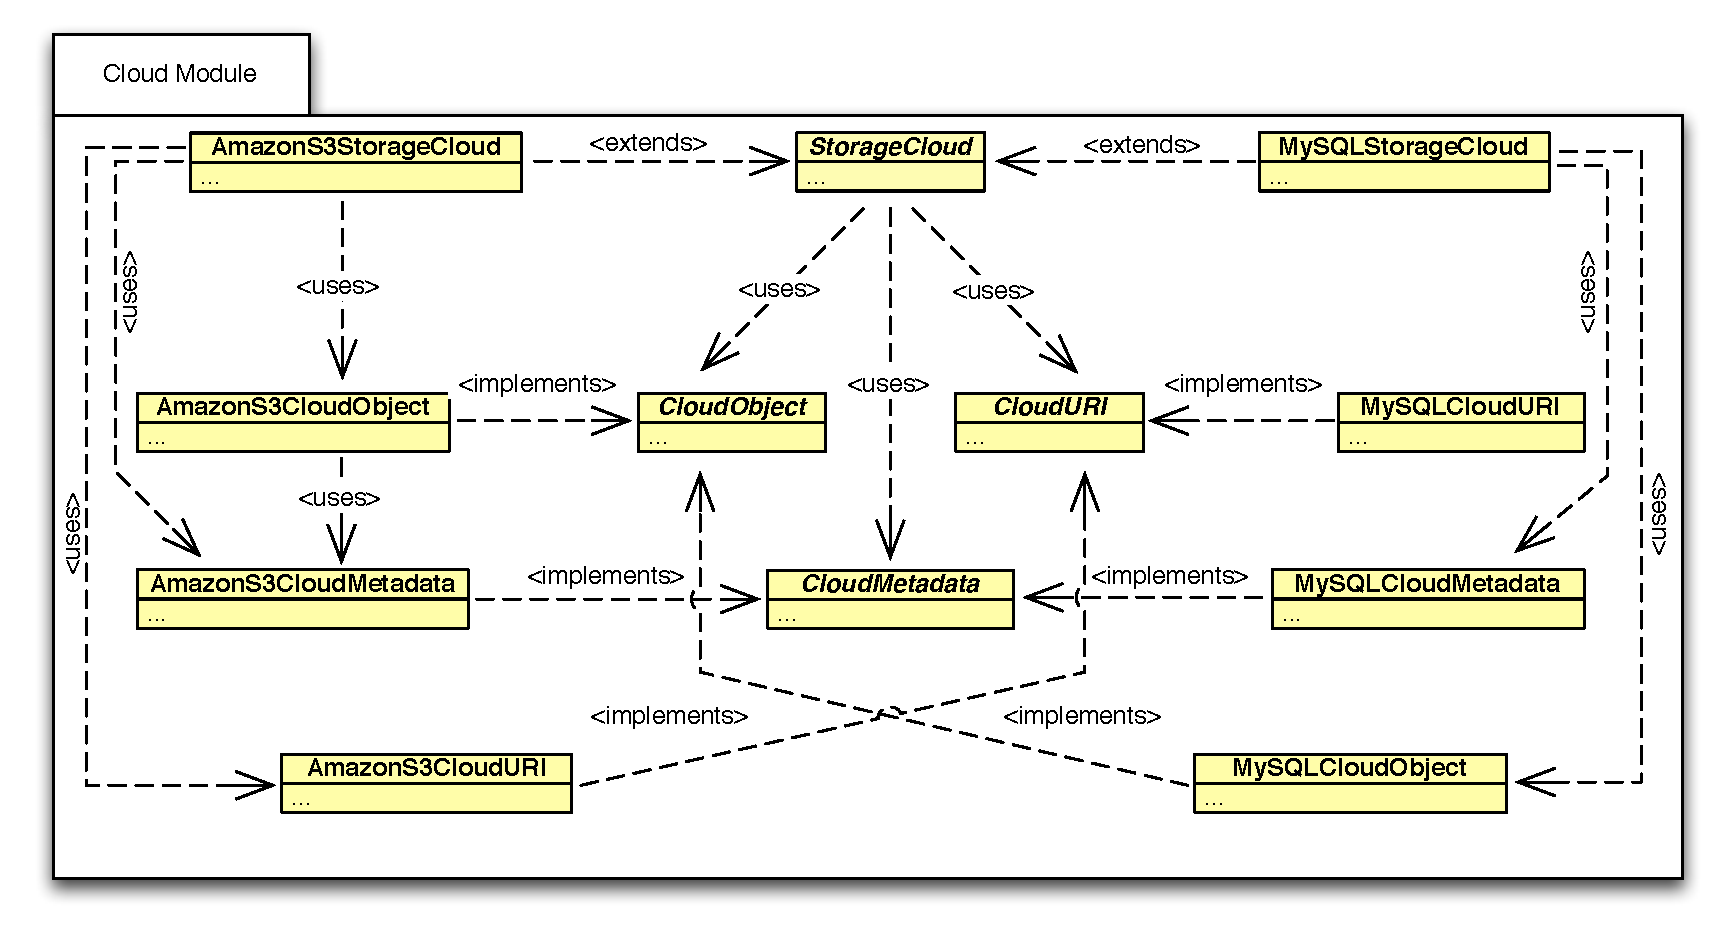
\includegraphics[width=\textwidth]{cloudypeer-cloudhelper-relations.pdf}
  \caption{Relations between classes of the \cloudhelper module}
  \label{fig:cloudypeer-cloudhelper-relations}
\end{figure}

\begin{figure}[h!]
  \centering
  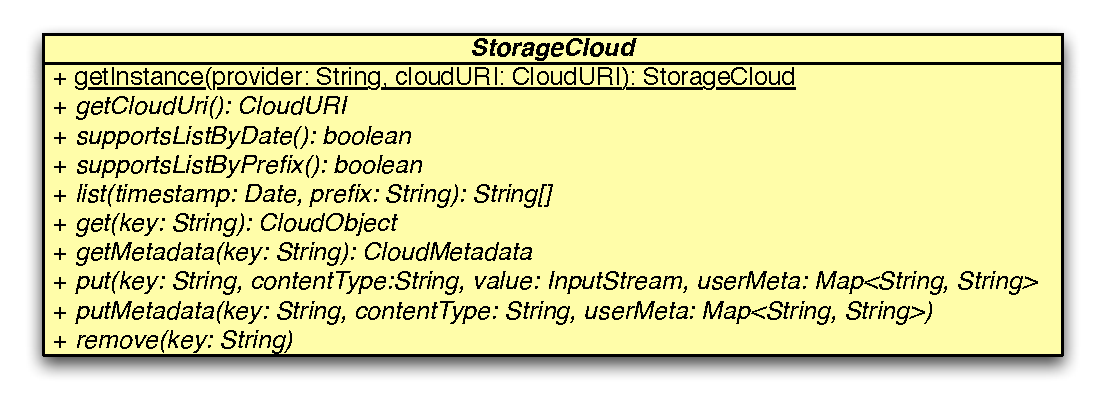
\includegraphics[width=\textwidth]{cloudypeer-cloudhelper-classdiagram.pdf}
  \caption{\texttt{StorageCloud} public \api}
  \label{fig:cloudypeer-cloudhelper-class}
\end{figure}

\ \\
The framework distribution ships two built-in \cloudhelper implementation
respectively for \textit{Amazon Simple Storage Service} and a
\textit{MySQL} backed \cloud service. The former is built upon
the official \textit{Amazon AWS SDK for Java}~\cite{AWS4Java} and it's
configured under the ``amazons3'' provider name, the latter
exploits the \textit{MySQL Connector/J}~\cite{MySQLConnectorJava} and
it's made available via the the ``mysql'' provider name.

The \textit{MySQL} \cloud is compatible with the one supported by
\grapes hence allowing using the same instance for both the
\peersampling and the actual storage. Table~\ref{tbl:mysql-cloud}
shows the base schema which a table must adhere to in order to being
used as a \cloud.

\begin{table}[H]
  \centering
  \begin{tabular}{|l|l|}
  \hline
  Field & Type \\
  \hline
  \hline
  cloud\_key & VARCHAR PRIMARY KEY \\
  cloud\_value & BLOB \\
  cloud\_timestamp &  INT UNSIGNED \\
  cloud\_content\_md5 &  VARCHAR(32) \\
  cloud\_content\_length &  INT UNSIGNED \\
  cloud\_content\_type & VARCHAR \\
  counter & INT UNSIGNED \\
  \hline
  \end{tabular}
  \caption{Schema of a \cloud enabled \textit{MySQL} table}
  \label{tbl:mysql-cloud}
\end{table}

\section{\textit{Store} module}
This module represents a key component of the \cloudypeer architecture
as it is responsible for all the storage-related tasks. As can be seen
by the extensive \api shown in figure
\ref{fig:cloudypeer-store-class}, such operations range from simple
listing and management duties to much more complex procedures aimed at
efficiently resolving differences between instances.

\begin{figure}[h!]
  \centering
  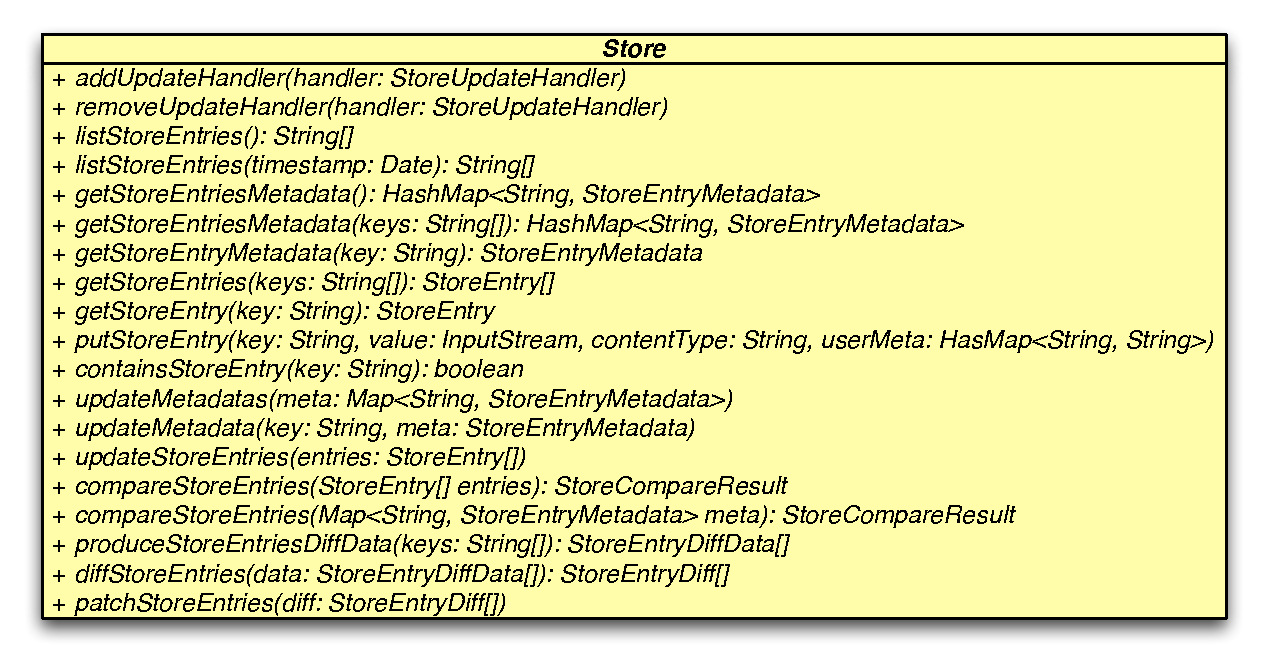
\includegraphics[width=\textwidth]{cloudypeer-store-classdiagram.pdf}
  \caption{\texttt{Store} public \api}
  \label{fig:cloudypeer-store-class}
\end{figure}

The former kind of operations are quite intuitive and for the most
part should not require additional comments. The only noteworthy
detail is that the version of \textit{listEntries} without parameters
has a peculiar behavior: the returned values may represent only a
partial view of the entire entries: specifically the ``active''
portion. The definition of ``active'' is application dependent and
expresses some innate property of the domain. For instance in a news
distribution scenario it may be based on time constraint as it's likely
that users are not interested in news which are too old.

Shifting the focus to the more complex operation, let's look at the
two variants of
\textit{compareStoreEntries}: these methods compare the \texttt{Store}
state against an array of entries and compile a report which specifyies
two entries' set. The first contains all the entries
which are \textit{fresher} on the local instance while the second embodies
the ones that should be updated due to being old or unknown.

Such information is of major importance to resolve the differences between
\texttt{Store} instances: this can be done either by replacing the old
entry with the fresher one or by updating only the portion of data
 which is changed. The second method is based on the
concept of \textit{diff} and \textit{patch}: the two entries are
compared and a list of the differences is computed (diff),
subsequently the oldest entry is updated by replaying the listed
modification (patch).

Remembering that we're working in a \ptop scenario an immediate
problem arises: we cannot transfer the whole entry to perform the
diff or this would nullify the purpose of the procedure. Similarly
we cannot maintain a record of all the remote instances states to
locally compute differences, as the
\ptop nature of the system would quickly render such records outdated
and thus useless. The only
viable approach is for the source \texttt{Store} to produce some data
which enables the remote instance to compute the differences.

For example a simple strategy is to divide the data in chunks and
compute an hash value for each of them. Once a remote instance receives
the list of hashes, it can compute its hashes and then
compare the two results. An even better approach would be to use some
\textit{rolling  checksum}~\cite{Rsync} scheme.
The \api enables this line of action via the functions:
\textit{produceStoreEntriesDiffData}, \textit{diffStoreEntries} and
\textit{patchStoreEntries}.

The last feature provided by the \textit{Store} module is represented
by the interface \texttt{StoreUpdateHandler} which allows the event
driven notification of storage changes.

\begin{figure}[h!]
  \centering
  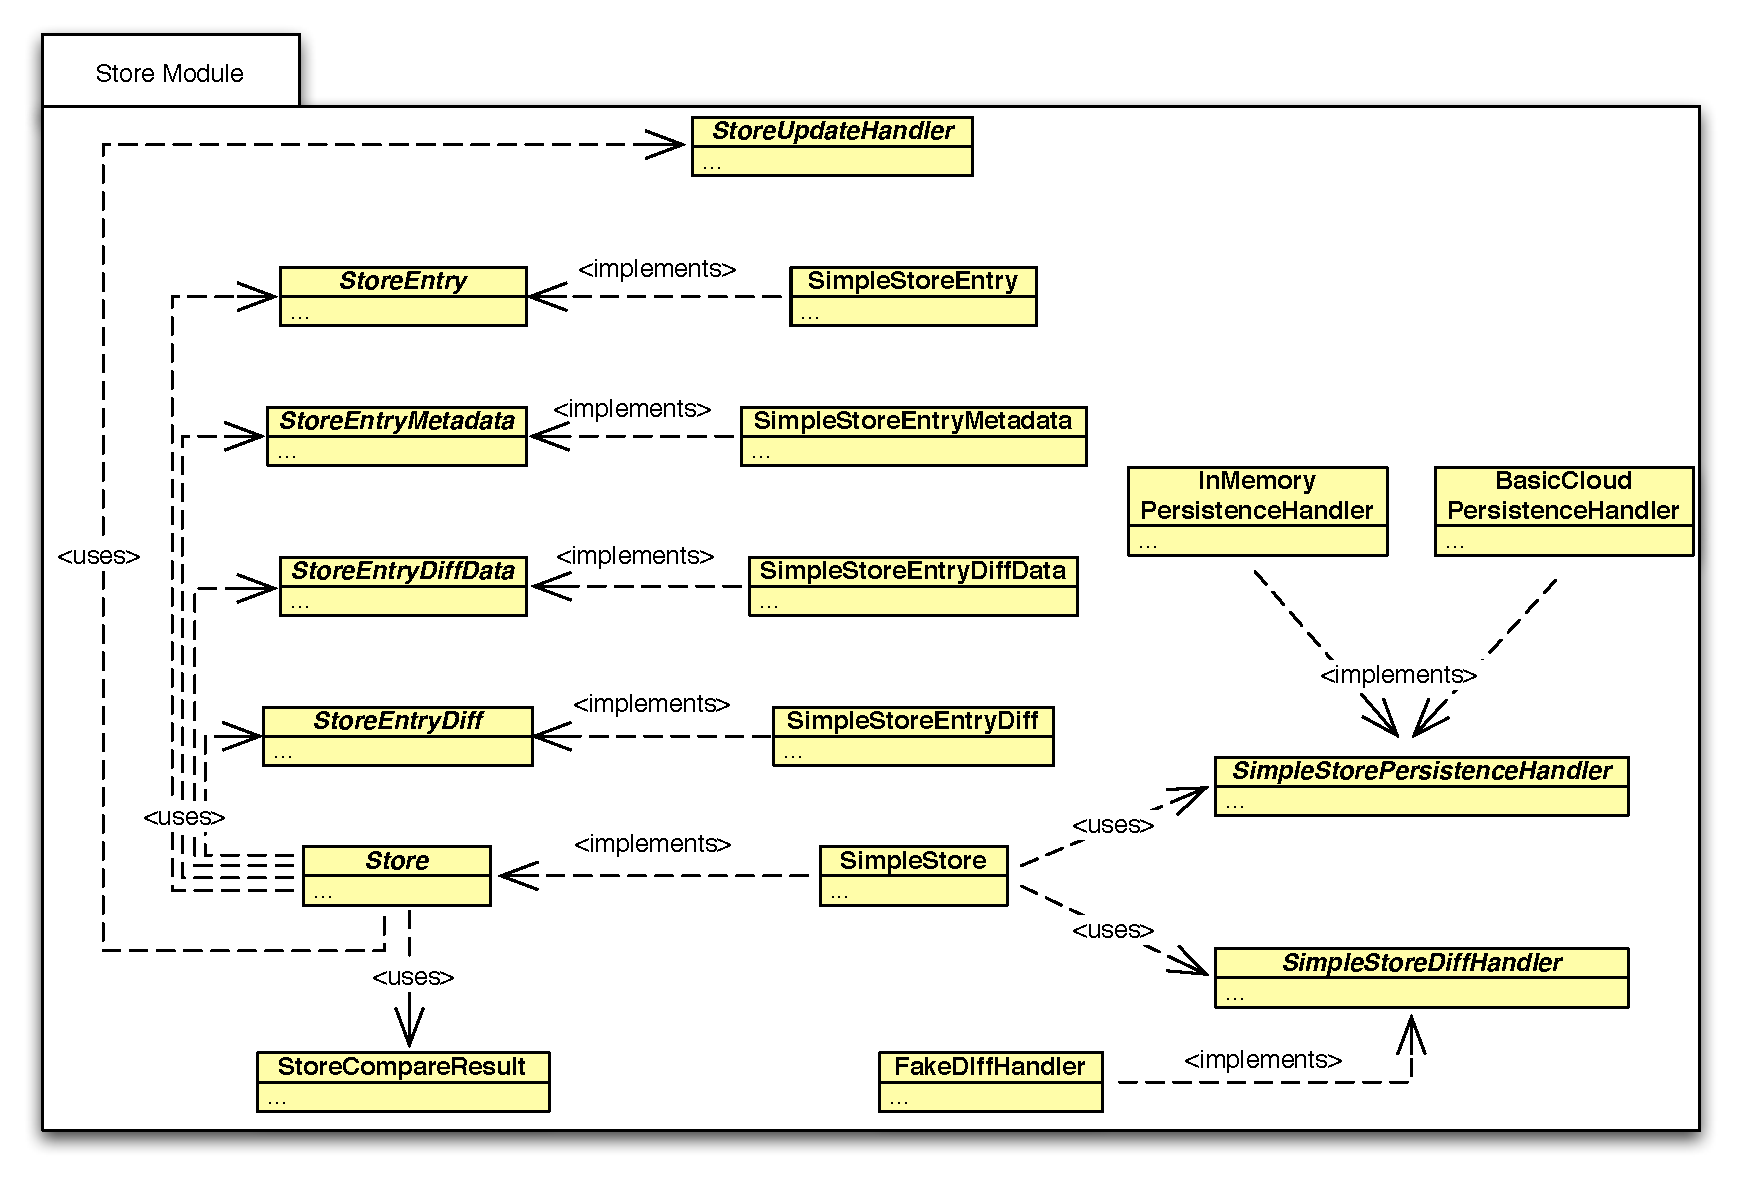
\includegraphics[width=\textwidth]{cloudypeer-store-relations.pdf}
  \caption{Relations between classes of the \cloudhelper module}
  \label{fig:cloudypeer-store-relations}
\end{figure}

\ \\
As shown in the module overview proposed in
figure~\ref{fig:cloudypeer-store-relations} the framework is
distributed with a built-in \texttt{Store} implementation providing
most of the basic functionality while delegating only the management of the
actual persistence and \textit{diff} strategy. Developers can design their
own persistence layer by subclassing
\texttt{Simple\-Store\-Persistence\-Class} and developing \textit{write}, \textit{read} and
\textit{list} procedures. Two default implementations of this class are
made available: the first exploits the \cloudhelper and uses a \cloud
instance as storage, the second instead keeps all its entries in
memory and is intended as a local storage implementation.

Similarly, different \textit{diff} schemes can be implemented by
extending \texttt{Simple\-Store\-Diff\-Handler} and writing
an implementation of the three action describes above. Given that
these are strictly dependent on the application scenario, the
framework only ships with a \textit{fake} component which makes the
\texttt{Store} compatible with protocols exploiting this
functionality, relaying however on the transmission of the complete data.

\section{\emph{Peer sampling} protocols}
All the components which are employed by \cloudypeer to provide
support for \peersampling protocols are enclosed in a module called
\textit{Peer Sampling}. The diagram of the various classes and their
relations is proposed in figure~\ref{fig:cloudypeer-peersampling-relations}.

\begin{figure}[h!]
  \centering
  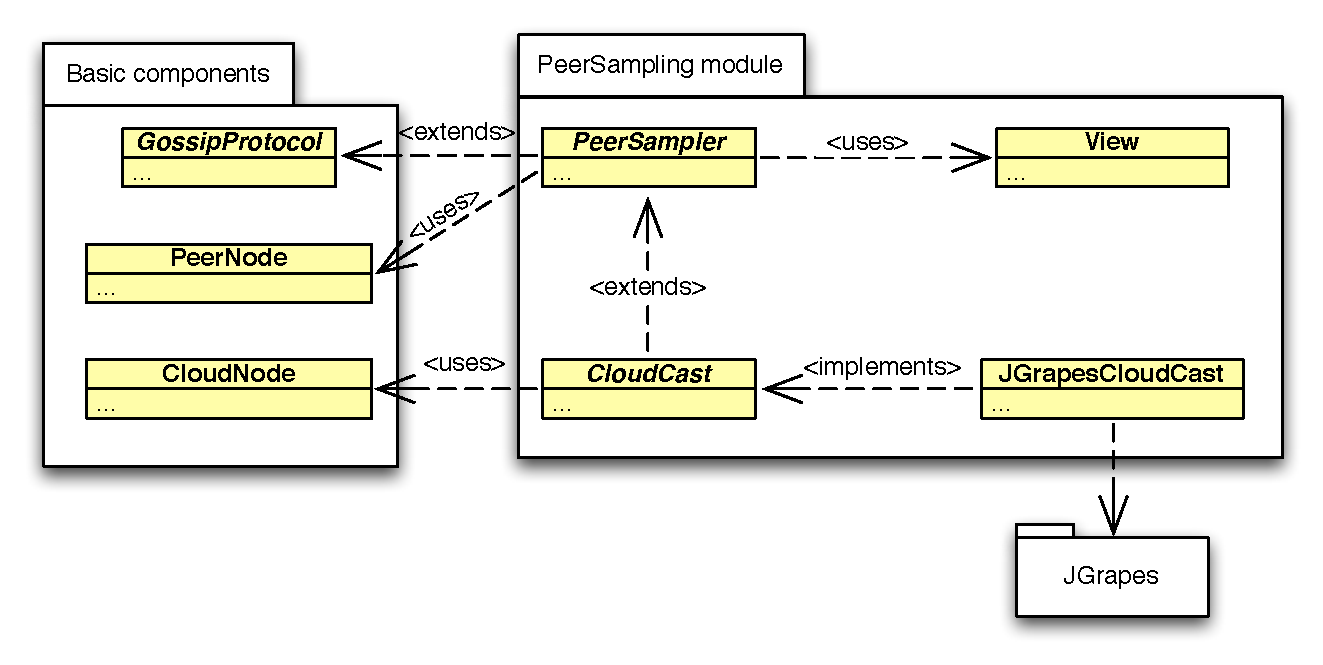
\includegraphics[width=\textwidth]{cloudypeer-peersampling-relations.pdf}
  \caption{Relations between classes of the \peersampling module}
  \label{fig:cloudypeer-peersampling-relations}
\end{figure}

Given that this work has been mainly concerned with implementing a
\cloudcast based application, the only available protocol at this time
is represented by \texttt{CloudCast}. However support for
conventional protocols can be added simply by subclassing
\texttt{PeerSampler}. The task if further simplified by the fact that
\grapes already implements some of them, hence it's sufficient to
write a wrapper which just performs the data conversion and delegates
all the real work to the library. Indeed this very strategy is adopted
by the built-in \texttt{JGrapesCloudCast} implementation.

The \api provided to developers can be seen in the diagram proposed in
figure~\ref{fig:cloudypeer-peersampling-class}. All the basic
functionalities are inherited by \texttt{GossipProtocol}, hence the
\texttt{PeerSampler} only need to define the standard methods to
interact with the network partial \view. As can be seen by looking at
the \texttt{CloudCast} definition, all that is left for the actual
protocol classes to specify is the instantiation mechanism and
possibly methods to manage additional parameters.

\begin{figure}[h!]
  \hspace{-50pt}
  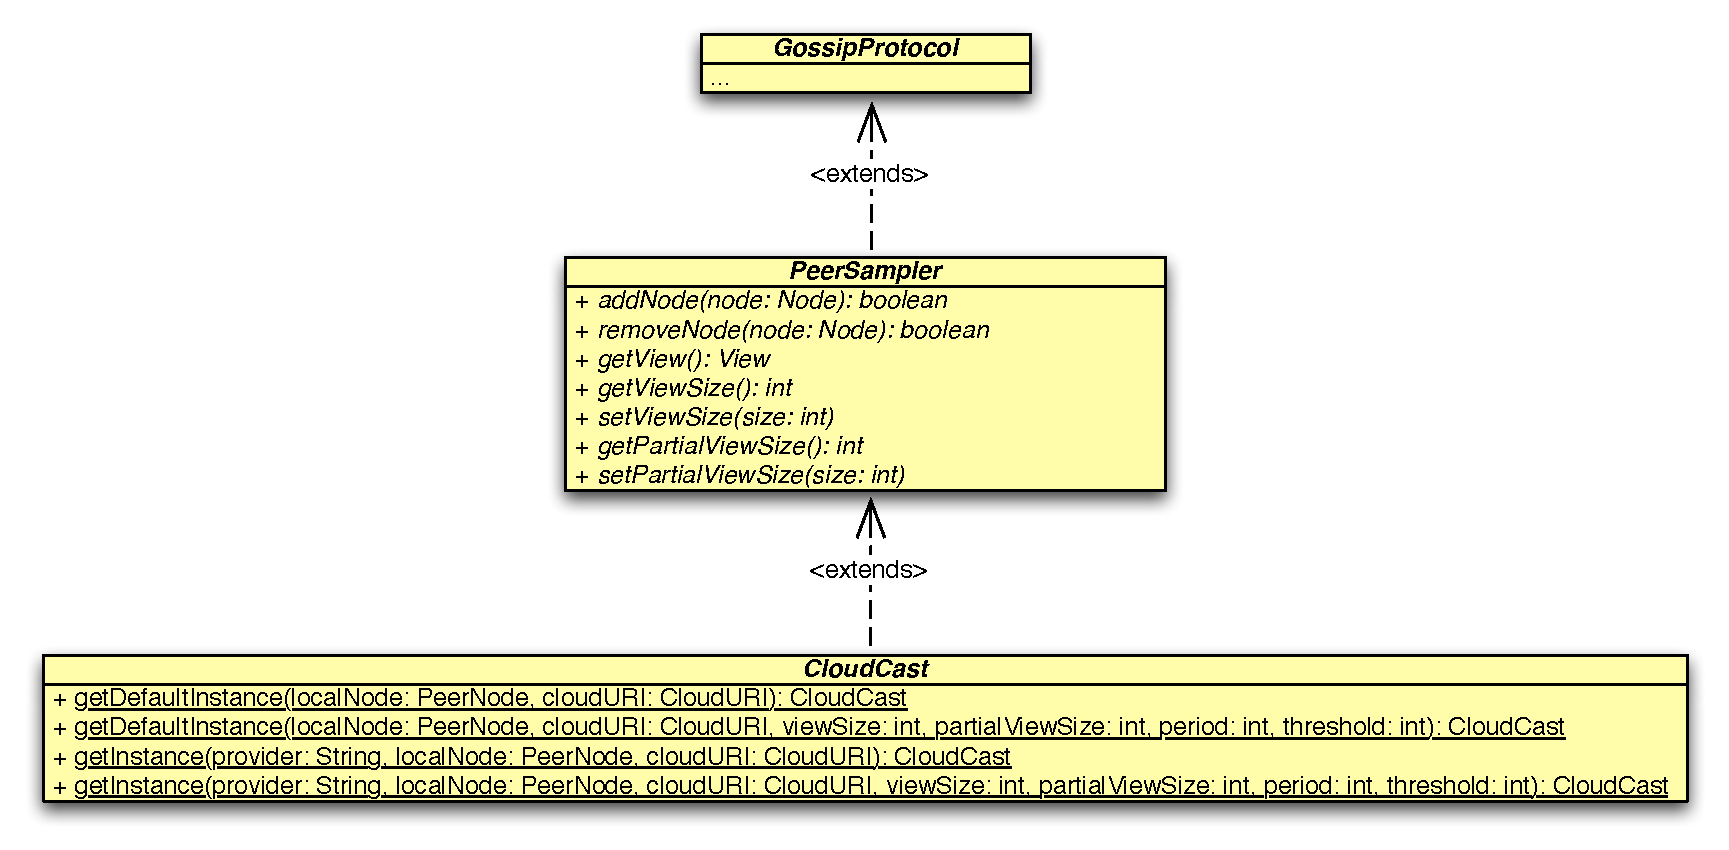
\includegraphics[width=1.3\textwidth]{cloudypeer-peersampling-classdiagram.pdf}
  \caption{Details of the \texttt{CloudCast} \api}
  \label{fig:cloudypeer-peersampling-class}
\end{figure}

The offered \api is simple enough that a detailed description is not
appropriate in this context. More information on the meaning of the
various parameters can be found in the \javadoc of the various
classes.

\section{\emph{Epidemic broadcast} protocols}
The module that concludes this overview of the \cloudypeer
architecture is the one providing the infrastructure for the \epidemic
protocols.

\begin{figure}[h!]
  \centering
  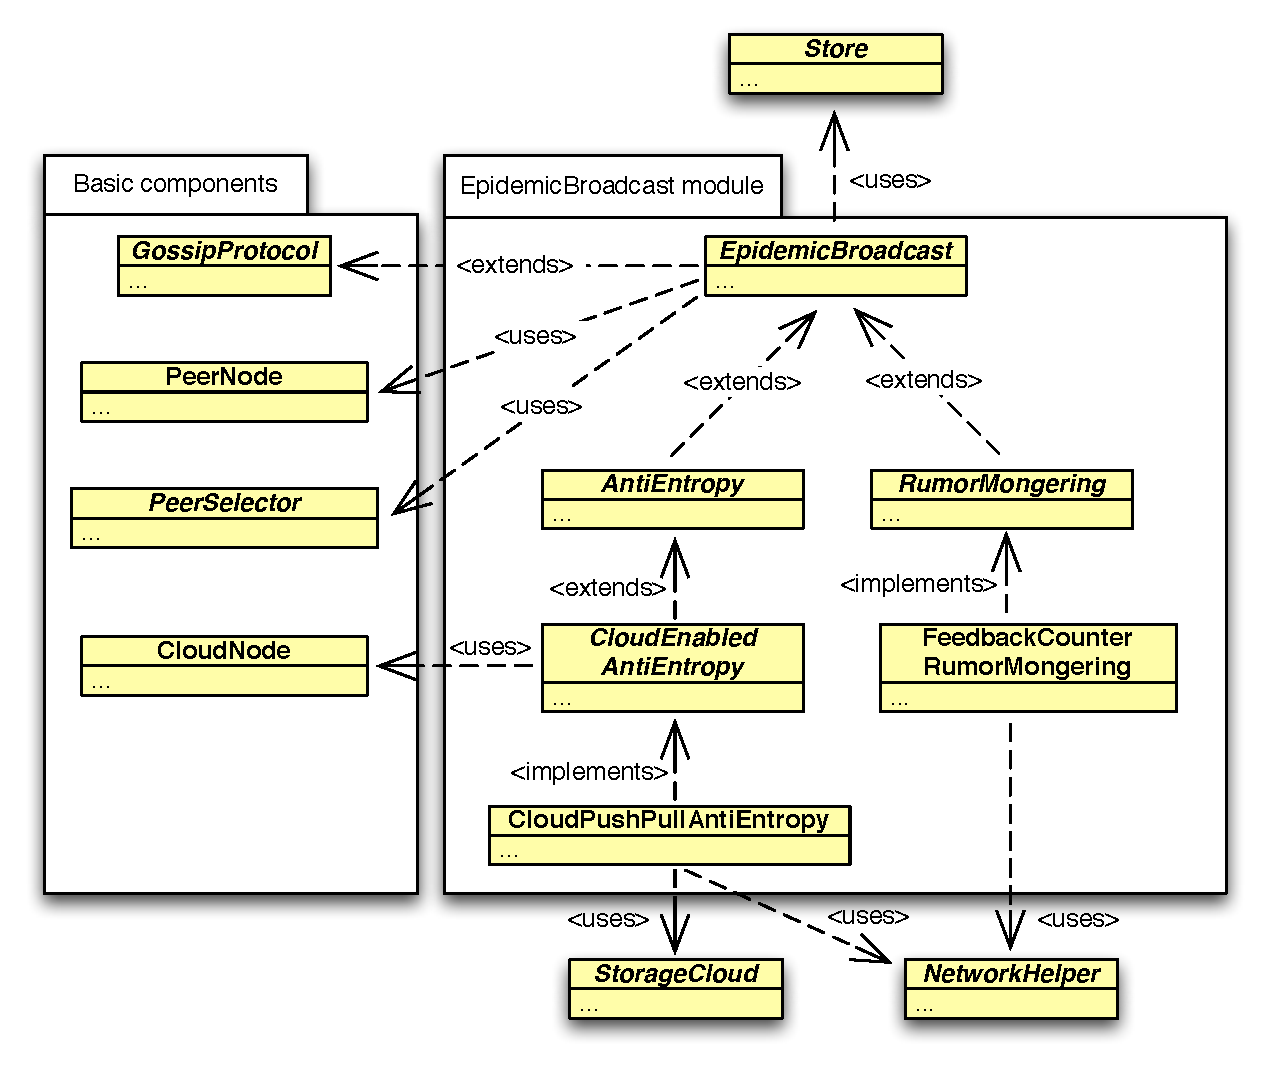
\includegraphics[width=\textwidth]{cloudypeer-epidemicbroadcast-relations.pdf}
  \caption{Relations between classes of the \textit{Epidemic
      broadcast} module}
  \label{fig:cloudypeer-epidemicbroadcast-relations}
\end{figure}

The structure of the module is for itself quite simple and intuitive as
can be noted analyzing the diagram shown in figure
\ref{fig:cloudypeer-epidemicbroadcast-relations}. By taking into
account the picture as a whole however it can be note that the module
display a strong dependence factor. Indeed here it's possible to see how
the \api infrastructure thus far defined comes into play to simplify
the development of high-level protocols. By heavily relaying on the
other modules, the implementation of the two \epidemic broadcast
protocols result very simple and most importantly general.

Figure~\ref{fig:cloudypeer-epidemicbroadcast-class} shows the main
classes forming the module's architecture and details the exposed
methods. Once again most of the functionalities are inherited from
\texttt{GossipProtocol} and the remaining one should be already clear
from previous considerations; refer to the \javadoc for further details.

\begin{figure}[h]
  \hspace{-50pt}
  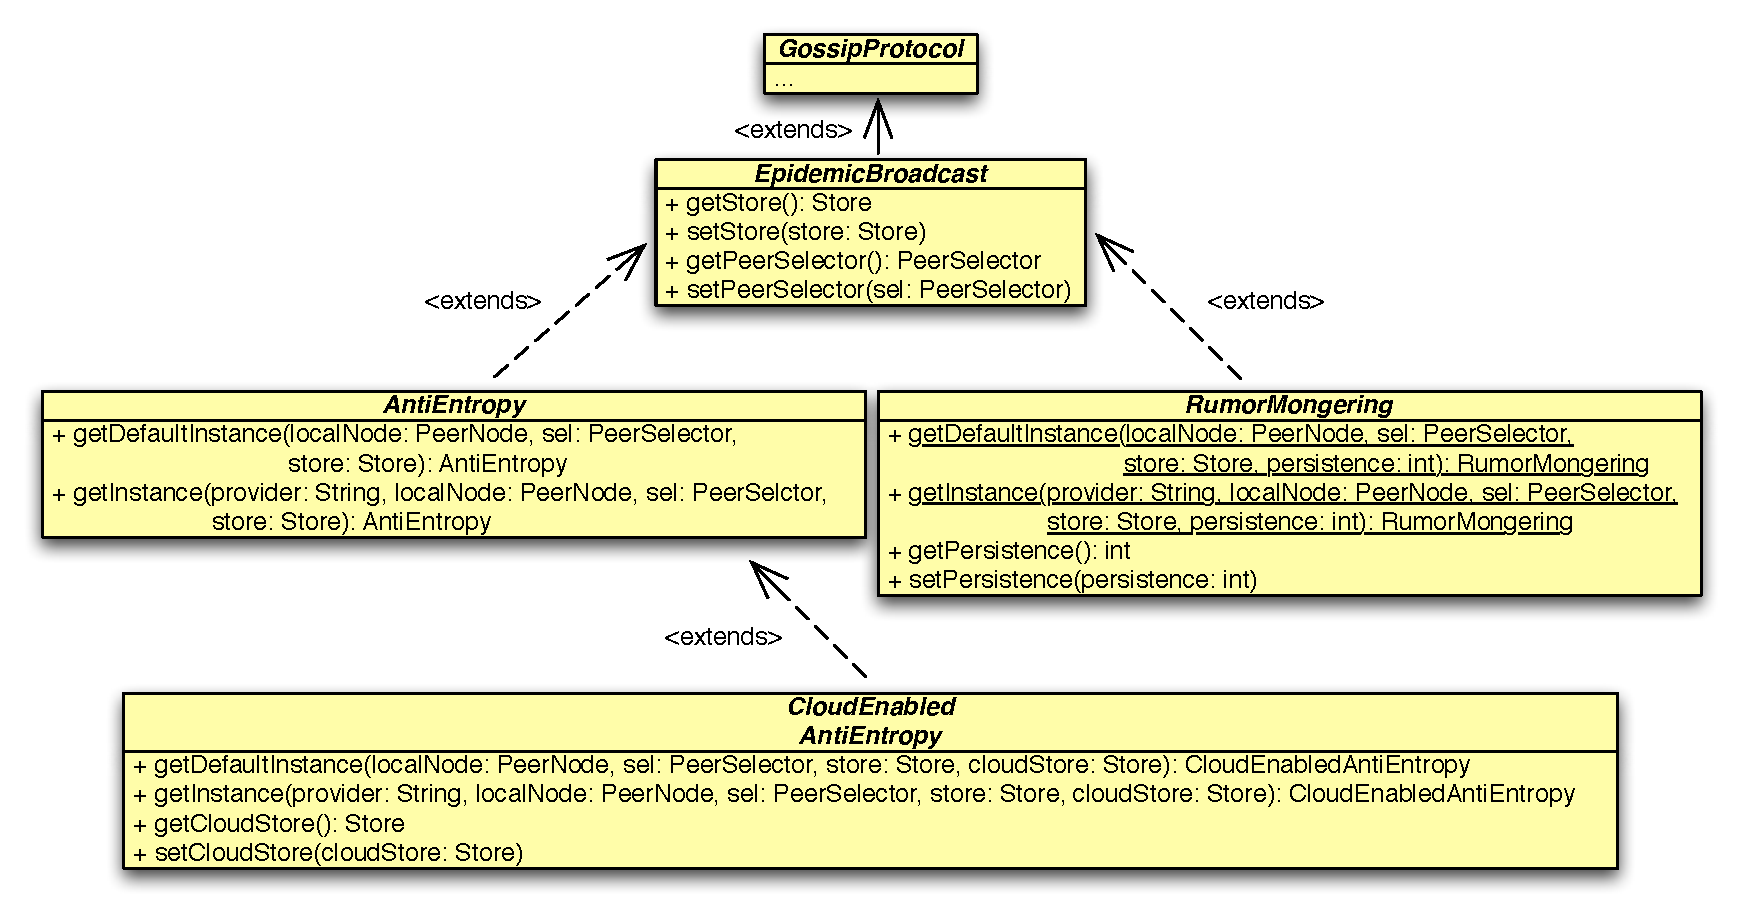
\includegraphics[width=1.3\textwidth]{cloudypeer-epidemicbroadcast-classdiagram.pdf}
  \caption{Details of the \textit{Epidemic broadcast} module \api}
  \label{fig:cloudypeer-epidemicbroadcast-class}
\end{figure}

At the current state the framework provides two built-in protocol
implementations: \texttt{CloudPushPullAntiEntropy} and
\texttt{FeedbackCounterRumorMongering}. As their names suggest, the
former uses a \PUSHPULL\ strategy and displays support for the \cloud while
the latter implements a standard \rumormongering algorithm with peer
feedback and termination based on counter.
Even though the implementations follow closely what has been stated in
section~\ref{sec:epidemicbroadcast}, in the following paragraphs will be
explained in detail the procedures executed with the intent of
clarifying the interactions with the various \cloudypeer components.

\begin{figure}[h]
  \centering
  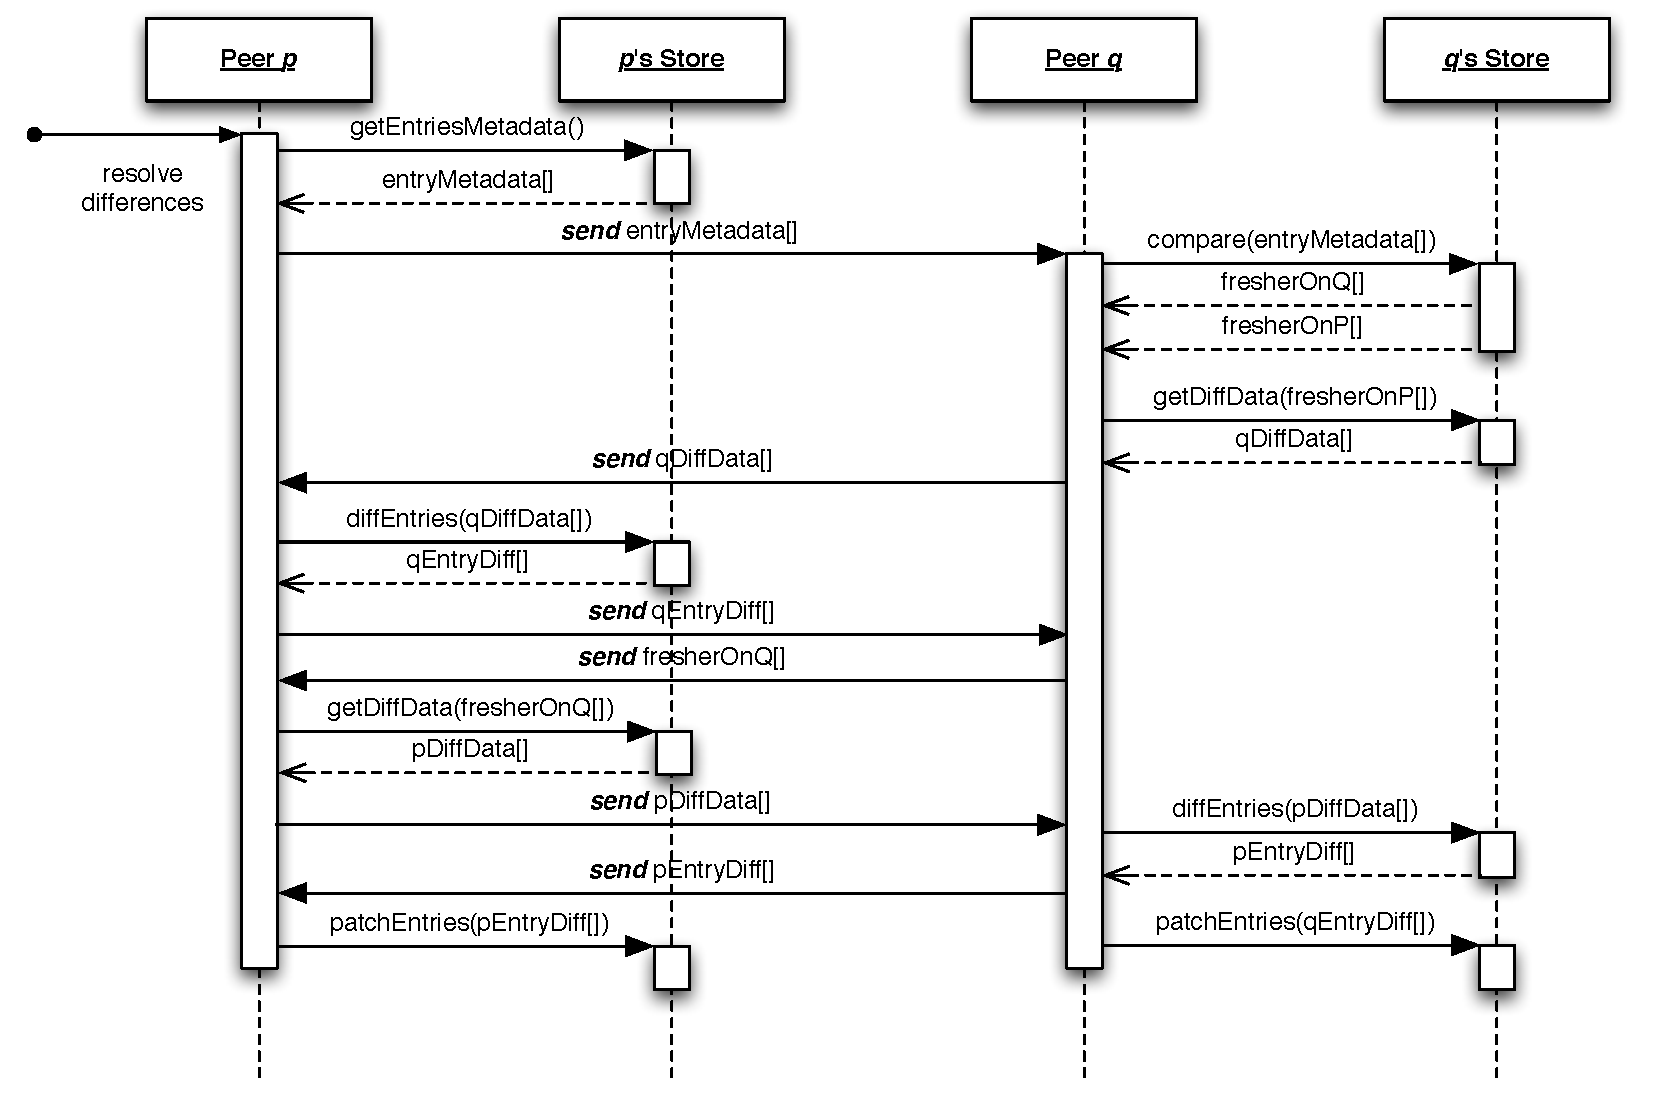
\includegraphics[width=\textwidth]{cloudypeer-antientropy-peer.pdf}
  \caption{Sequence diagram of an \antientropy\ cycle involving a remote
    peer (\PUSHPULL\ strategy)}
  \label{fig:cloudypeer-sequence-antientropy-peer}
\end{figure}

Figure~\ref{fig:cloudypeer-sequence-antientropy-peer} shows an
\antientropy cycle between two peers. As a first operation the
initiating peer $p$ queries its \texttt{Store} for the entries'
metadata. These are sent, using the \networkhelper, to the remote
peer $q$ which delegates to its \texttt{Store} instance the job of
analyze them. As a result of this operation, $q$ obtains two lists:
one for the entry to be pulled and one for the entry to be pushed.
At this point $q$ produces and sends the data which  $p$ uses to generate
the \textit{diff} information needed to patch $q$'s \texttt{Store}. The
same process is subsequently performed with switched roles concluding
the messages exchange between the two peer which at this point can
update their respective \texttt{Store} and conclude the execution.

\begin{figure}[h]
  \centering
  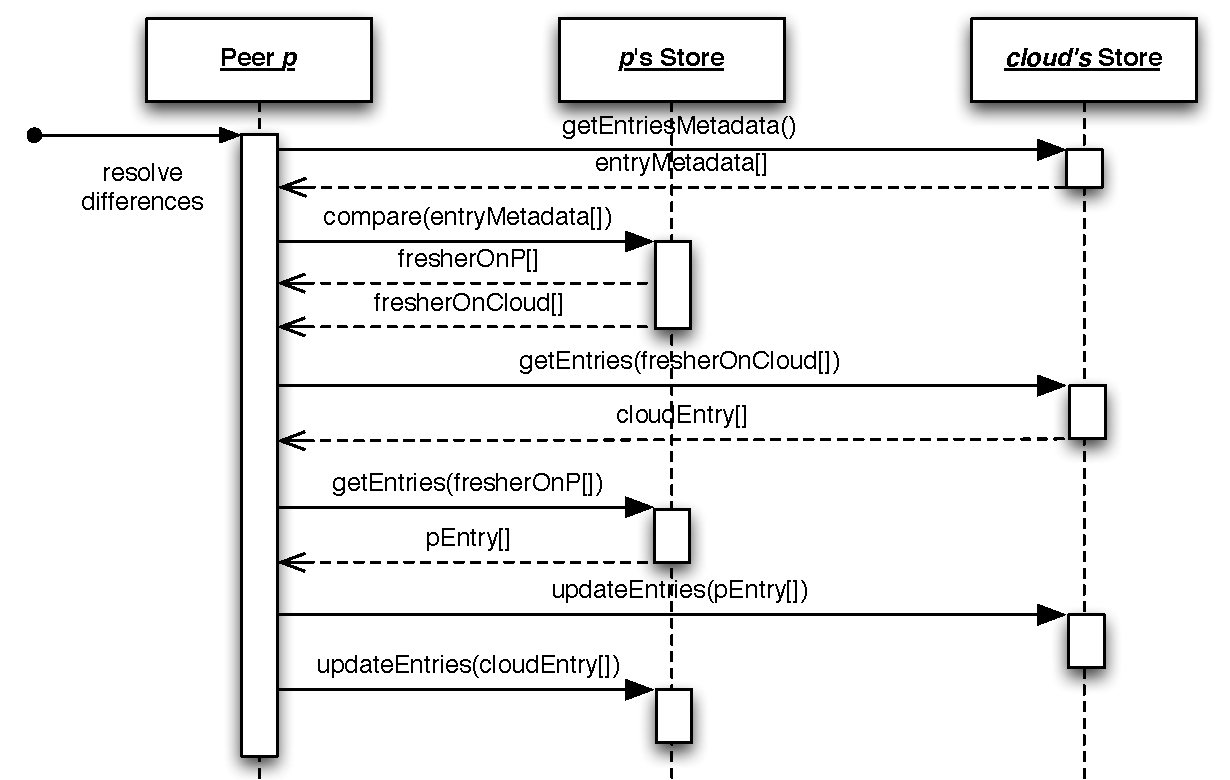
\includegraphics[width=\textwidth]{cloudypeer-antientropy-cloud.pdf}
  \caption{Sequence diagram of an \antientropy\ cycle involving the
    \cloud\ (\PUSHPULL\ strategy)}
  \label{fig:cloudypeer-sequence-antientropy-cloud}
\end{figure}

\ \\
\noindent Figure~\ref{fig:cloudypeer-sequence-antientropy-cloud} displays the
actions executed when an \antientropy cycle involves the \cloud. As
can be seen all the computation is performed by the initiating peer
which orchestrates the entire exchange. The followed steps are similar
to the ones described for the previous case, however the passive
nature of the \cloud causes a major difference: the whole data is
transferred in both the direction. This fact means that data exchanged
with the \cloud may display much higher bandwidth costs with respect
to the same exchange between two peers. Fortunately, as will be
discussed later, this problem doesn't have an high impact on the
overall cost.

\ \\
\noindent The last diagram, shown in
figure~\ref{fig:cloudypeer-sequence-rumormongering}, illustrate the
behavior of the \rumormongering implementation. Here the similarities
with the first case are much more evident. Indeed the higher half of the
diagram display exactly the same operation. The few differences are
represented by the fact that updates only flow in one direction and
more importantly that the triggering factor isn't the firing of a
timer but instead the notification by the \texttt{Store} which a new
update is available.

\begin{figure}[H]
  \centering
  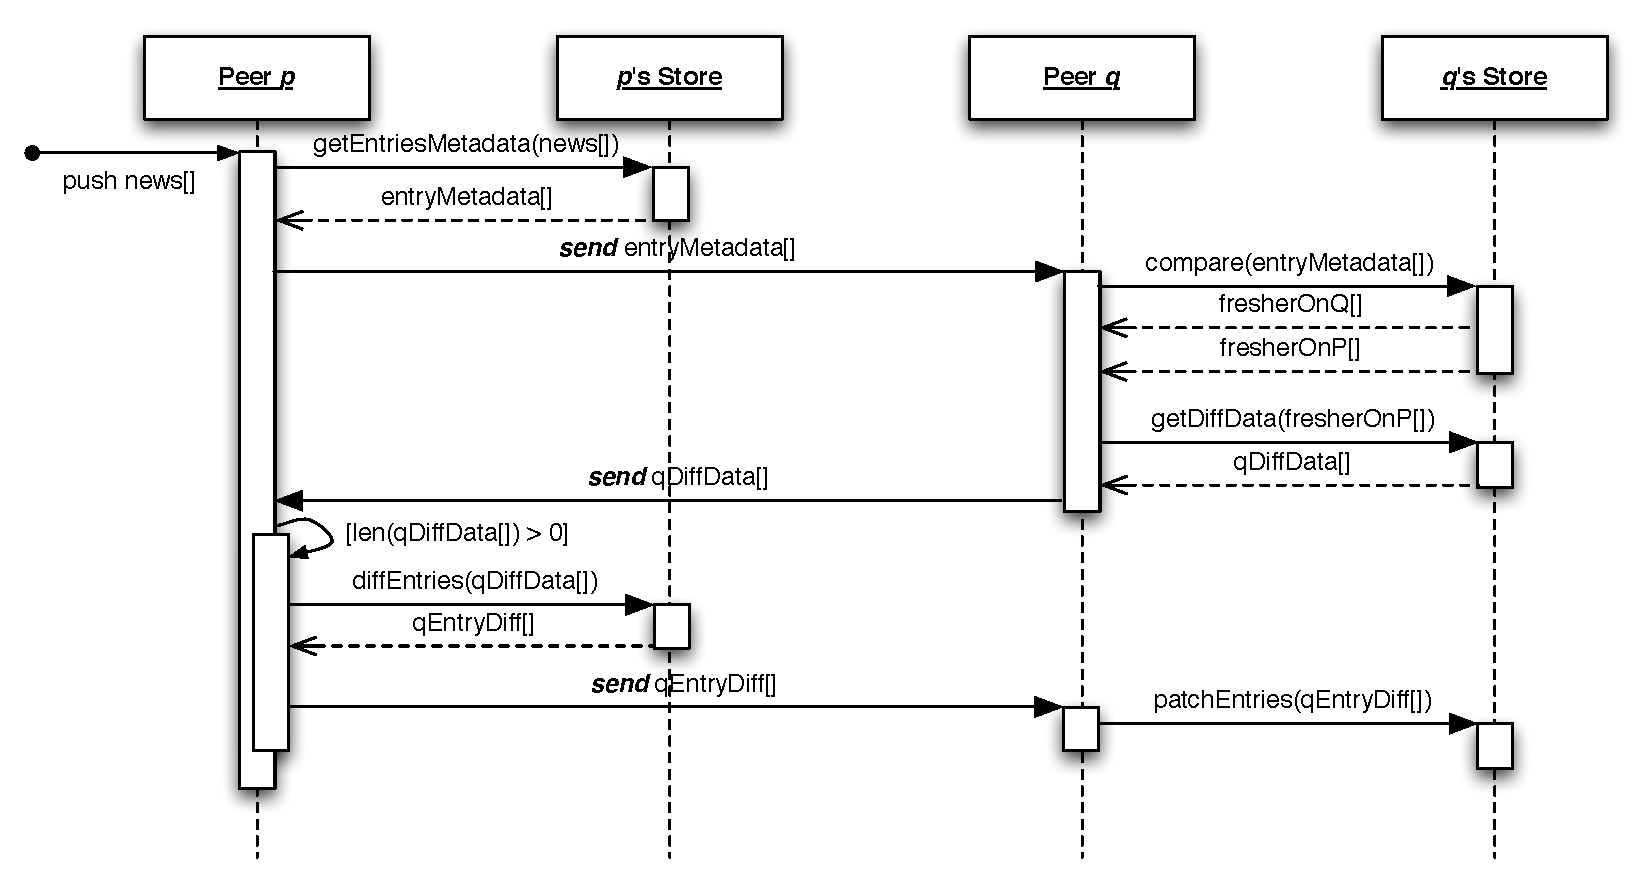
\includegraphics[width=\textwidth]{cloudypeer-rumormongering.pdf}
  \caption{Sequence diagram of a \rumormongering\ cycle}
  \label{fig:cloudypeer-sequence-rumormongering}
\end{figure}

\clearpage
\section{Building and using the framework}
To conclude the analysis of the framework in this section will be
explained how \cloudypeer can be compiled and used by developers to
write their \ptop applications.

As for the other library developed during the course of this thesis,
the code is available via a \github repository~\cite{cloudypeer-repo}
with the last version available at the time of this writing tagged
by \thesistag.

The distribution already contains all the \textit{Java} dependencies
included \jgrapes. To built the framework is sufficient to invoke the
\texttt{dist} target of the \textit{ant} build file. This command will
generate a directory named \texttt{dist} containing the \textit{jar}
files of \cloudypeer and all the other dependencies.

At this point the framework can be used by simply adding the various
\textit{jars} to the \textit{Java classpath}. To successfully use the
\jgrapes based \peersampling protocol implementation however the
\textit{Java} property \texttt{java.library.path} must be configured
to include the directory containing all the native libraries used by
\jgrapes. Such a directory is produced during the building process of
\jgrapes under the name \texttt{dist}.

The listing available in figure~\ref{lst:cloudypeer-example-app}
provide a fully working, even if minimal, application based on \cloudypeer.
As can be noted the amount of code needed by the developer to setup
the \cloudcast infrastructure is really small: skipping comments,
blank lines and variable declarations only $19$ operations are
required.

This example only serves the role of demonstrating the convenience
offered by the framework, more elaborated examples are available in
the codebase of \cloudypeer under the \texttt{test} pckage.

\begin{figure}[H]
  \lstinputlisting[language=Java,basicstyle=\footnotesize,numberstyle=\footnotesize,numbers=left,frame=leftline]{code/cloudypeer-example.java}
  \hspace{-100pt}
  \caption{Skeleton of a simple application exploiting \cloudypeer}
  \label{lst:cloudypeer-example-app}
\end{figure}

\section{Evaluation}
In this section are proposed some results showing the
effectiveness of the framework in terms of \textit{news}
distribution.

Let's start by analyzing the delays in the delivery of \textit{news}
considering a dynamic scenario. Figure
\ref{fig:cloudypeer-oscillating-delays} match plot
\ref{fig:cloudcast-sim-oscillating-delays} which is reproposed here
for convenience. Due to lack of resources it hasn't been possible to
perform the test under exactly the same conditions: the maximal network
size had to be limited to $170$ nodes instead of $500$. However all
the other parameters have been maintained: the experiment has lasted 2
days with a new
\textit{news} added each four hours. The \antientropy and
\rumormongering protocols have been configured with a period of
respectively $10$ and $1$ seconds.

As can be seen the delays obtained by the \cloudypeer implementation
are slightly smaller with respect to the ones recorded during the
simulation.
This variation can be partially attributed to
the different network sizes, however it's our opinion that the
improved result is achieved mostly thanks to the more elaborated
\rumormongering protocol which, exploiting peer's feedback, is more
effective in quickly diffusing updates.

\begin{figure}[H]
  \centering
  \subfloat[][\cloudypeer experiment]{
    \hspace{-70pt}
    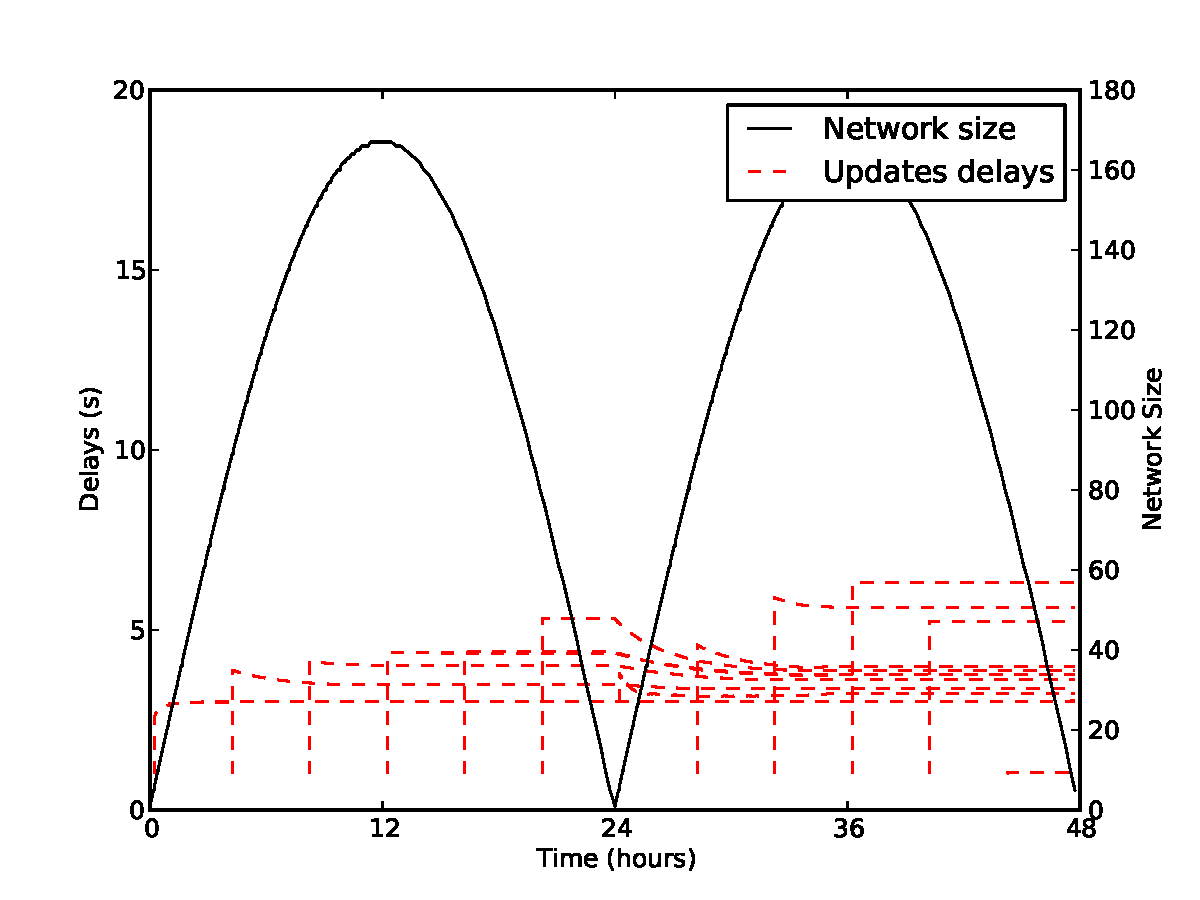
\includegraphics[width=240pt]{cloudypeer-oscillating-delays.pdf}
    \label{fig:cloudypeer-oscillating-delays}
  }
  \subfloat[][Simulated \cloudcast experiment]{
    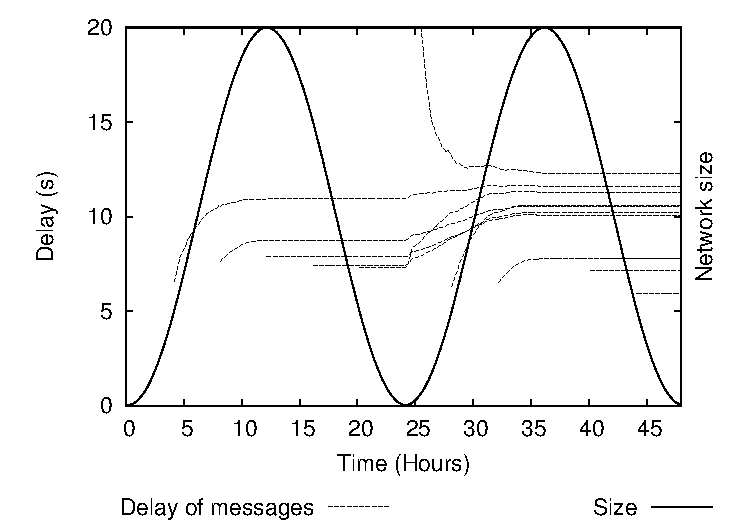
\includegraphics[width=240pt]{cloudcast-sim-oscillating-delays.pdf}
  }
  \caption{Progressive delays in message diffusion in a dynamic scenario}
  \label{fig:cloudcast-globa-delay}
\end{figure}

Another interesting measure of evaluation is represented by the
traffic generated by the system. In this case we're not interested
in the actual number of bytes exchanged but instead we focused our
analysis on the number of times each node \textit{pushes} some
data. The rationale behind this reasoning is that the framework allows
to easily change the actual network implementation and \textit{diff}
strategy, hence a measure influenced by these components wouldn't be
of much value.

The experiments have been setup to employ a network
which linearly grows up to a target size and exchanges \textit{news}
generated with a $5$ minutes period for a total duration of one hour.
Each configuration has been iterated $10$ times and the displayed
values represent the aggregated statistics.
Due to lack of time and resources it hasn't been possible to
experiment on networks with a more significative size; future works may
fill this gap by providing more exhaustive results.

The data about node's exchanges shown in table~\ref{tbl:pushed-news}
displays a predictable scenario: the majority of the
work is carried out by the \rumormongering protocol while \antientropy
has a much smaller impact. Of more interest is the data regarding the
number of news that have been pushed by \cloud, presented in
table~\ref{tbl:cloud-news}: the mean values are really small compared
to the total amount of updates transferred during the whole
experiment. In particular it can be noted how the contribution of the
\cloud never surpasses the $2\%$ of the total. This demonstrates once
again the effectiveness of the \cloudcast approach and at the same
time proves the correctness of the implementation.

\begin{table}[h!]
  \centering
  \begin{tabular}{|c|c|c|c|c|c|c|c|c|}
  \hline
  Size & Protocol & Avg & Var & Min & Q1 & Q2 & Q3 & Max\\
  \hline
  \hline

  \multirow{2}{*}{32} &
        \antientropy & 3.32 & 5.45 & 0 & 1 & 3 & 5 & 11 \\

       &\rumormongering & 8.57  & 9.89 & 1 & 6 & 8 & 11 & 16\\

  \hline
  \multirow{2}{*}{64} &
        \antientropy & 2.87 & 4.32 & 0 & 1 & 3 & 4 & 10\\

      & \rumormongering & 9.08 & 10.93 & 2 & 7 & 9 & 11 & 21\\

  \hline
  \multirow{2}{*}{128} &
        \antientropy & 2.52 & 4.15 & 0 & 1 & 2 & 4 & 14\\

      & \rumormongering & 9.35 & 13.28 & 1 & 7 & 9 & 12 & 22 \\

  \hline
  \multirow{2}{*}{160} &
        \antientropy & 2.80 & 5.66 & 0 & 1 & 2 & 4 & 16\\

      & \rumormongering & 9.027 & 13.54 & 1 & 6 & 9 & 11 & 24 \\
  \hline
  \end{tabular}
  \caption{Statistic on the \textit{news} pushed by the \epidemic
    broadcast protocols}
  \label{tbl:pushed-news}
\end{table}

\begin{table}[h!]
  \hspace{-30pt}
  \begin{tabular}{|c|c|c|c|c|c|c|c|c|c|}
  \hline
  Size & Updates \# & Cloud \% & Cloud Avg & Cloud Var & Min & Q1 & Q2 & Q3 & Max\\
  \hline
  \hline
  32 & 384 & 1.45\%  & 5.59 & 5.44 & 2 & 3 & 6 & 8 & 8 \\
  64 & 768 & 0.73\% & 5.79 & 7.76 & 3 & 3 & 5 & 9 & 10 \\
  128 & 1536 & 1.2\% & 19.19 & 29.76 & 11 & 13 & 21 & 24.5 & 26\\
  160 & 1920 & 1.72\% &33.03 & 44.12 & 26 & 27 & 30 & 40.5 & 44 \\
  \hline
  \end{tabular}
  \caption{Statistic on the \textit{news} obtained via the \cloud}
  \label{tbl:cloud-news}
\end{table}

\chapter{CloudyRSS}
Simulations and small tests conducted in a controlled environment are a
good way to evaluate the effectiveness of complex infrastructures as the
one displayed by \cloudcast. However only data gathered via a
deployed system can provide a realistic picture.
Keeping this in mind, the final work performed during this thesis
has been directed to develop a simple yet realistic application based
on the \cloudypeer framework and exploiting the \cloudcast
architecture.

News distribution, in the form of \textit{RSS} feeds, has been chosen as
the target scenario since it perfectly fits the proposed
approach: it features a central component with a dynamic set of
updates to be distributed to a potentially huge collection of nodes.
The literature shows multiple works where \ptop techniques
have been applied to the \textit{RSS} distribution
problem~\cite{P2PFeedDelivery}
\cite{AttackResilientP2PFeedDissemination}
\cite{SimpleSecurityP2PFeedDissemination}, however to the best of our
knowledge none tries to conciliate the central nature of the problem
with the \ptop component.

The result of this effort is an application called \cloudyrss which
allow standard \textit{RSS reader} software to fetch their news via a
\cloudcast based system.

\begin{figure}[h!]
  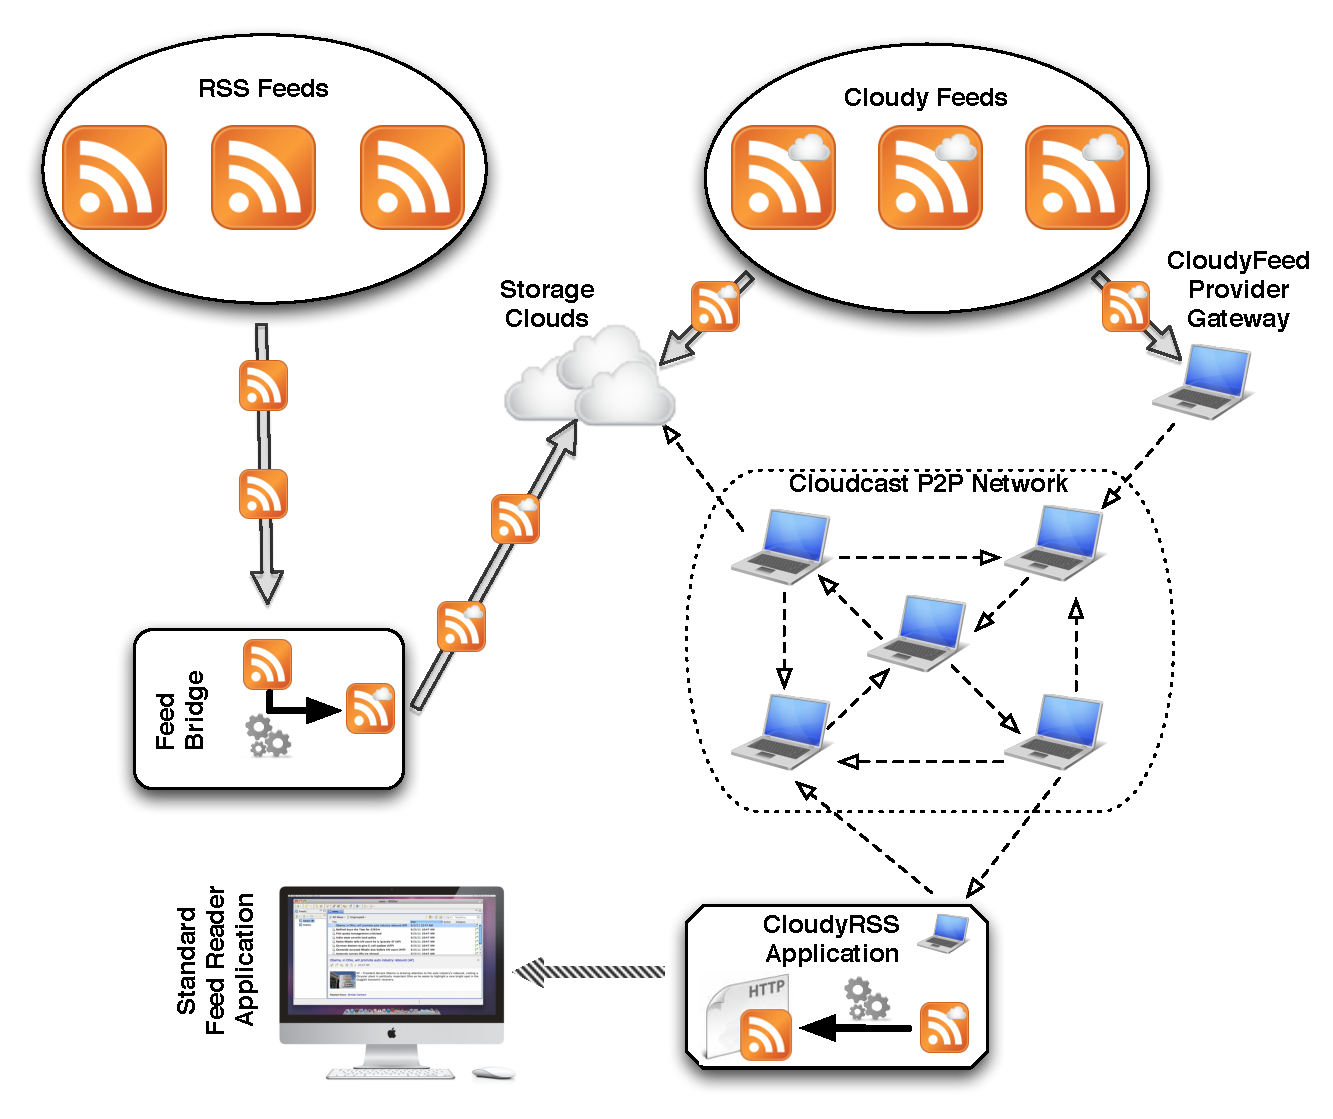
\includegraphics[width=\textwidth]{cloudyrss-architecture.pdf}
  \caption{Architectural overview of \cloudyrss}
  \label{fig:cloudyrss-architecture}
\end{figure}

Figure~\ref{fig:cloudyrss-architecture} shows a general overview of
the system. As can be noted, the news sources are divided in two
categories. The first is represented by the \cloudyrss-aware sources
which are fully integrated in the system: their updates are distributed
by placing them on the cloud and/or by employing a gateway node
responsible of starting the epidemic diffusion.
The second category embodies all the standard \textit{RSS} feed
sources: these are not directly involved in the architecture; instead their
updates are collected by an entity called \textit{Feed
  Bridge} which converts them in \cloudyrss compatible news and place
them on the cloud.

Once the updates are entered in the system, \cloudcast takes care of
delivering them to all subscribed nodes where they are converted back in
\textit{RSS} form and offered via a local web server instance to the
\textit{RSS reader} software of choice.

\begin{figure}[h!]
  \centering
  \subfloat[][\cloudyrss\ status window showing ``news'' feed URL]{
    \hspace{-70pt}
    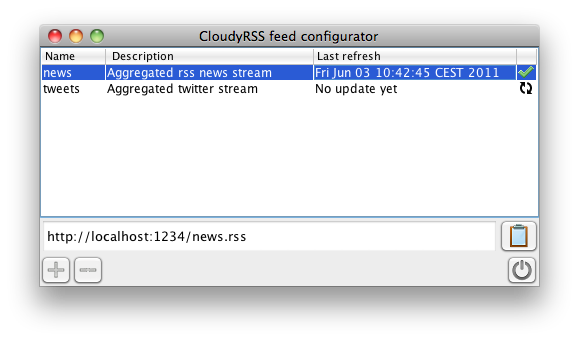
\includegraphics[width=240pt]{cloudyrss-main.png}
    \label{fig:cloudyrss-main}
  }
  \subfloat[][RssOwl properties window for feed ``news'']{
    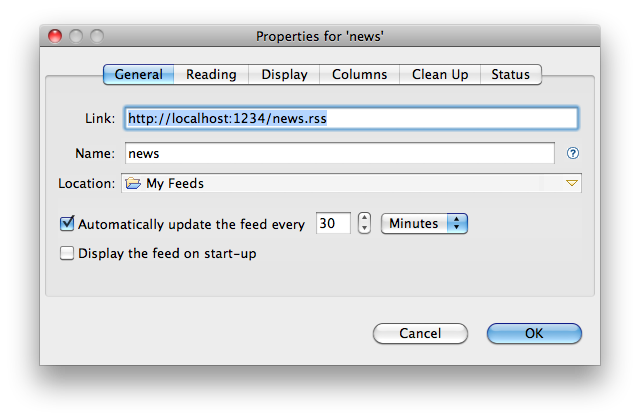
\includegraphics[width=240pt]{cloudyrss-properties.png}
    \label{fig:cloudyrss-properties}
  }
  \caption{Feeds' URLS configuration in an RSS reader}
  \label{fig:cloudyrss-feeds}
\end{figure}

\clearpage
Users can subscribe to a news feed by loading a
configuration file equivalent to the ``.torrent'' one used by
\textit{BitTorrent} softwares. Once the desired feed have been
added, the \textit{RSS reader} must be configured to use them.
Figures~\ref{fig:cloudyrss-main} and~\ref{fig:cloudyrss-properties}
shows this process: the URL of the \textit{RSS file} generated by
\cloudypeer is copied from the main application window and entered in
the feed configuration window of the \textit{RSS reader}.
The end result is that the news obtained via the \cloudcast system are
transparently displayed in the \textit{RSS reader} as shown in
Figure~\ref{fig:cloudyrss-view}

Thanks to this system is possible to setup experiments confronting the
costs of distributing the \textit{RSS} file with the
\cloudcast based system with respect to the standard strategy. The actual
planning and realization of such tests is however out of the scope of
this work and thus will not be analyzed further.

Once again the code of \cloudyrss is available via a \github
repository~\cite{cloudyrss-repo} with the last version at the time of
this writing tagged with \thesistag.

\begin{figure}[h!]
  \hspace{-40pt}
  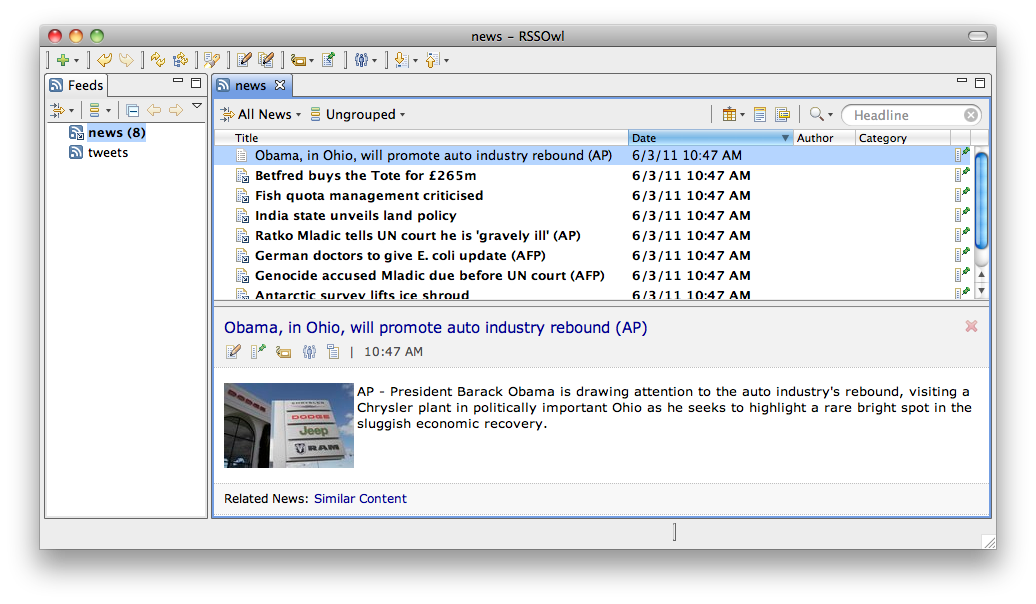
\includegraphics[width=1.2\textwidth]{cloudyrss-view.png}
  \caption{RssOwl main windows showing the ``news'' feed obtained
    through \cloudyrss}
  \label{fig:cloudyrss-view}
\end{figure}

\chapter{Conclusions}
This thesis describes the efforts aimed at creating a
working implementation of the \cloudcast architecture, which have
culminated in the creation of the \cloudypeer framework. In achieving
this result a series of other accomplishments have been reached. First
and more importantly, the original \cloudcast infrastructure has been
improved with the addition of a recovery mechanism directed to
guarantee the stability of the underlying peer sampling
protocol. An additional noteworthy endeavor has been targeted to resolve
bugs and extend the functionalities of the \grapes toolkit in order
to make it suitable to serve as foundation.

The general performances of the implementation have been analyzed and
confronted with the ones proposed in the original
paper~\cite{Cloudcast}. Moreover, the enhancements to the protocol's
algorithms have been evaluated, showing how the system benefits from
their presence and at the same time how the additional overhead
is overall negligible.

The \cloudypeer framework has been described in detail, explaining how
the various components interact with each other and how developers can
easily extend its behavior to fit their need. This analysis was aimed at
proving the generality and ease of use features
central to the framework's design.

Finally, a concrete example application called \cloudyrss has been presented,
which proves the viability of the proposed approach and the correctness of the
described implementation.

\paragraph{Future work}
There are a number of interesting problems that have not been covered
in this thesis due to lack of time. Concerning the \cloudcast
architecture itself, one of the results proposed in the original
paper~\cite{Cloudcast} has shown that a major portion of the expense is
caused by the peer sampling. An easy, yet effective, way to reduce its
impact would be to study alternative \textit{bootstrapping} strategies
not based on the cloud. Examples of such tactics are:
\begin{itemize}
  \item Employing local and/or web based peer
    caches~\cite{GnutellaWebCache}~\cite{P2PVPN}
  \item Probing the network for entry
    points~\cite{BootstrappingP2P}~\cite{BootstrappingP2PLocality}
    ~\cite{DecentralizedBootstrappingP2P}
    \item Exploiting \textit{Dynamic DNS}
      services~\cite{DecentralizedBootstrapping}
\end{itemize}
Furthermore, the system could be made more realistic by investigating
ways to take advantage of the security feature offered by cloud
provider such as Amazon in terms of authentication, access control and
versioning~\cite{AmazonS3DevGuide}.

Moving our focus on the actual implementation, an obvious extension
would be the addition of more cloud storage service
providers and a greater variety of peer sampling protocols. Moreover
further work should be made to better adapt the
cloud descriptors handling to the peculiarities of the \grapes's
cache design.

In conclusion, a final effort which would greatly enhance
the performances of the system is the development of a better \networkhelper
implementation for the \cloudypeer framework, possibly relaying on the
correspondent module of \grapes.

\addcontentsline{toc}{chapter}{Bibliography}
\bibliography{bibliography}{}
\bibliographystyle{unsrt}
\end{document}
